\documentclass[pdflatex,sn-mathphys-num,iicol]{sn-jnl}

\usepackage[T1]{fontenc}
\usepackage{amsmath,amssymb}
\usepackage{algorithm}
\usepackage{algpseudocode}
\algrenewcommand\algorithmicrequire{\textbf{Input:}}
\algrenewcommand\algorithmicensure{\textbf{Output:}}
\algrenewcommand{\algorithmiccomment}[1]{\hfill(#1)}
\usepackage{booktabs}
\usepackage{placeins}
\usepackage{array}
\usepackage{graphicx}
\usepackage{tikz}
\usepackage{pgfplots}
\pgfplotsset{compat=1.17}
\usetikzlibrary{arrows.meta,calc,positioning,patterns}
\hypersetup{hypertexnames=false}
\renewcommand{\topfraction}{0.9}
\renewcommand{\bottomfraction}{0.8}
\renewcommand{\textfraction}{0.07}
\renewcommand{\floatpagefraction}{0.8}
\renewcommand{\dbltopfraction}{0.9}
\renewcommand{\dblfloatpagefraction}{0.8}
\setcounter{topnumber}{3}
\setcounter{bottomnumber}{2}
\setcounter{totalnumber}{5}
\setcounter{dbltopnumber}{3}
\newcommand{\ci}[3]{\begin{tabular}[c]{@{}c@{}}$#1$\\{}[$#2$, $#3$]\end{tabular}}
\newcommand{\cib}[3]{{\boldmath\ci{#1}{#2}{#3}}}
\newcommand{\cit}[3]{\begin{tabular}[t]{@{}c@{}}$#1$\\{}[$#2$, $#3$]\end{tabular}}
\newcommand{\cibt}[3]{{\boldmath\cit{#1}{#2}{#3}}}
\newcommand{\scl}{SCL}
\newcommand{\aob}{AOB}
\newcommand{\twol}[2]{\begin{tabular}[c]{@{}l@{}}#1\\#2\end{tabular}}

\makeatletter
\def\email#1{\global\advance\emailcnt by 1\relax
\if@corauemail
  \ifx\corrauthemail\@empty\g@addto@macro\corrauthemail{\textcolor{blue}{#1}}%
  \else\g@addto@macro\corrauthemail{;\ \textcolor{blue}{#1}}\fi
\else
  \ifx\authemail\@empty\g@addto@macro\authemail{\textcolor{blue}{#1}}%
  \else\g@addto@macro\authemail{;\ \textcolor{blue}{#1}}\fi
\fi}
\makeatother

\begin{document}

\title[Self-Calibrating Control Layer for Multi-Object Trackers]{Training-Free Self-Calibrating Control Layer for Heterogeneous Multi-Object Trackers}

\author*[1]{\fnm{Ahmed Gouda} \sur{Ismail}}\email{a7medgouda1@gmail.com}
\author[2]{\fnm{Tarek Ahmed} \sur{Mahmoud}}\email{tarek.mohamed@eui.edu.eg}
\author[1]{\fnm{Mohamed S.} \sur{Mohamed}}\email{mohamedms@mtc.edu.eg}

\affil*[1]{\orgdiv{Computer Engineering and Artificial Intelligence Department}, \orgname{Military Technical College}, \orgaddress{\city{Cairo}, \country{Egypt}}}
\affil[2]{\orgdiv{Computer Engineering Department}, \orgname{Egypt University of Informatics}, \orgaddress{\city{Cairo}, \country{Egypt}}}

\abstract{Multi-object trackers rely on score thresholds tuned for one detector. When the detector is replaced, retrained, or compressed, its scores shift, and the tuned thresholds silently stop fitting. This paper proposes a training-free self-calibrating control layer (\scl{}) between an unchanged detector and tracker. \scl{} splits the logits of recent scores twice with Otsu's method and classifies the stream as clean or noisy, without labels or future frames. Its novelty is selective, host-aware adaptation. On clean streams it keeps the tracker's scores and lowers a threshold only if it would reject the confident detections; on noisy streams it selects and rescores the detections and sets the thresholds. It acts through four published tracker settings and passes on weak detections that continue tracks, so one frozen configuration serves single-stage and two-stage trackers. It was evaluated on seven trackers, four detection sources, and three datasets; changes are relative to the tracker alone. When detector scores were halved, two trackers fell to zero higher order tracking accuracy (HOTA); with \scl{} both recovered at least 97\% of it. With a replacement detector, RT-DETR-L, \scl{} raised the multiple object tracking accuracy (MOTA) of ByteTrack and BoT-SORT by 12.6\% and 16.3\% and cut their identity switches by 43\% and 47\%, respectively. It also raised the HOTA of PD-SORT, unseen during design, by 0.9\%, and kept four well-matched trackers within 0.1\%. \scl{} adds on average no more than 2.95 ms per frame on an ordinary processor, so a detector can be replaced or retrained without retuning the tracker.}



\keywords{multi-object tracking, tracking by detection, detector confidence calibration, online adaptation, Otsu thresholding, real-time image processing}

\maketitle

% --- sections/01_introduction
\section{Introduction}\label{sec:intro}

Multi-object tracking (MOT) finds every object of interest in a video and gives each one an
identity number (ID) that stays the same over time, for surveillance, driving, and drone systems
\cite{zhu2022visdrone}. In the tracking-by-detection design \cite{adzemovic2026survey}, a detector
returns candidate boxes with confidence scores, and a tracker links them into tracks
\cite{bewley2016sort,zhang2022bytetrack,cao2023ocsort}, using a box only if its score passes a fixed
threshold. A two-stage tracker, such as ByteTrack, also uses lower-score boxes in a second step to
continue tracks \cite{zhang2022bytetrack}; a single-stage tracker, such as OC-SORT, ignores every box
below one threshold \cite{cao2023ocsort}.

In real systems the detector is often replaced, retrained, or compressed, while the tracker keeps
thresholds set for another detector. Detector scores are not calibrated across models
\cite{kuppers2020detcalib}, so a new detector usually gives scores on a different scale. ByteTrack in
its official setting starts a track only from a box with a score of at least 0.7; when the scores
are halved, a car scored 0.9 gets 0.45, no track starts, and the higher order tracking accuracy
(HOTA) \cite{luiten2021hota} falls from 67.70 to 0 (Sect.~\ref{sec:shift}). Retuning every tracker
for every detector needs labels, adaptive-threshold methods are each built into one tracker
\cite{ma2023adaptivebytetrack,shim2024adaptrack,act2026adaptive}, score calibration needs labelled
data \cite{kuppers2020detcalib}, and adaptive inference methods learn their settings for one model
\cite{han2022dynamic}.

This paper presents a self-calibrating control layer (\scl{}) between a detector and a tracker that
are both kept fixed (frozen): their code, weights, and stored settings are unchanged. We call the
tracker that \scl{} serves the \emph{host}. The novelty of \scl{} is \emph{selective, host-aware
adaptation}. It is selective because it first decides, from the detector scores alone, whether the
stream fits the host: when most higher scores of recent frames form a clearly confident group, the
stream is clean and the host keeps its scores and thresholds; only when many scores are uncertain
does \scl{} choose the candidates, give them new scores, and set the thresholds. It is host-aware
because every action is expressed through four published settings of the host, the host contract
(Sect.~\ref{sec:contract}), so the same frozen rules serve single-stage and two-stage trackers.
With halved scores, \scl{} restored ByteTrack and OC-SORT from 0 to about 66 HOTA; with other
detectors, it raised the multiple object tracking accuracy (MOTA) of two-stage trackers by up to
24.7 points and cut their identity switches by 43\% to 56\%, while well-matched strong trackers
stayed within 0.06 HOTA points of their own accuracy. The main contributions are:
\begin{enumerate}
\item \emph{Selective adaptation:} a label-free, causal compatibility test (nested Otsu splits of
      recent logits and a whole-stream majority rule) that leaves a well-matched system as it is
      and corrects a mismatched one (Sects.~\ref{sec:calib}--\ref{sec:choice}).
\item \emph{Host-aware adaptation:} a host contract of four published values through which one
      fixed configuration serves unchanged single-stage and two-stage trackers, with a track-guided
      recovery of weak detections (Sects.~\ref{sec:rescue}--\ref{sec:contract}).
\item \emph{Evidence:} one frozen configuration evaluated on seven trackers, four detection sources,
      and three datasets, with paired bootstrap intervals, adaptive-threshold baselines, the
      published ACT method, an ablation, and a sensitivity analysis (Sect.~\ref{sec:results}), at
      about 3 ms per frame on a central processing unit (CPU) (Sect.~\ref{sec:discussion}).
\end{enumerate}

Section~\ref{sec:related} presents the datasets, evaluation metrics, and related work.
Section~\ref{sec:method} describes the proposed \scl{} framework, while
Section~\ref{sec:development} details its development and refinement. Section~\ref{sec:results}
presents the experimental results and evaluation. Finally, Sections~\ref{sec:discussion}
and~\ref{sec:conclusion} discuss the practical implications and summarize the main findings and
future research directions, respectively.
% --- sections/02_background
\section{Background and Related Work}\label{sec:related}

\subsection{Datasets}\label{sec:data}
\emph{MOT17} \cite{milan2016mot16} contains people filmed with static and moving cameras; as is
common, the second half of its seven training sequences, val-half (2,652 frames), is used for
evaluation \cite{zhang2022bytetrack}, with the published YOLOX-X detections \cite{ge2021yolox} at the
two published emission floors (lowest emitted scores) of 0.01 and 0.1. To study score changes
directly, these scores were also changed before the tracker by four order-preserving transforms:
cubing ($s^3$), halving ($0.5\,s$), and logit temperatures $T=2$ and $T=0.5$, which divide the logit
of each score (Sect.~\ref{sec:problem}) by $T$. \emph{KITTI tracking} \cite{geiger2012kitti} has 21
training sequences (8,008 frames) recorded from a car, scored on cars and pedestrians, and is used
with two other detectors, YOLOv8n \cite{jocher2023yolov8} and RT-DETR-L \cite{zhao2024rtdetr}.
\emph{UAVDT} \cite{du2018uavdt} contains drone videos of vehicles; its 20 test sequences (16,592
frames) are used with ByteTrack, YOLOv8n, and RT-DETR-L. MOT17 with four trackers, KITTI, and the
score transforms were development data. Two predeclared external trackers, PD-SORT and Hybrid-SORT,
were run once with the frozen configuration on their authors' MOT17 val-half detections, and the
held-out UAVDT test split was run once after a written plan. Each external host was checked against
its authors' number: EXACT within 0.2 HOTA points, CLOSE within 1.0.

\subsection{Evaluation metrics}\label{sec:metrics}
HOTA \cite{luiten2021hota}, the main metric, balances finding the objects and keeping their
identities,
\begin{equation}
\mathrm{HOTA}=\frac{1}{19}\sum_{\alpha}\sqrt{\mathrm{DetA}_\alpha\,\mathrm{AssA}_\alpha},
\label{eq:hota}
\end{equation}
where $\mathrm{DetA}_\alpha$ and $\mathrm{AssA}_\alpha$ are the detection and association accuracy
at the localization threshold $\alpha=0.05,0.10,\dots,0.95$.

MOTA \cite{bernardin2008clear} and IDF1 \cite{ristani2016idf1} are
\begin{align}
\mathrm{MOTA}&=1-\frac{\mathrm{FN}+\mathrm{FP}+\mathrm{IDS}}{\mathrm{GT}},\label{eq:mota}\\
\mathrm{IDF1}&=\frac{2\,\mathrm{IDTP}}{2\,\mathrm{IDTP}+\mathrm{IDFP}+\mathrm{IDFN}},\label{eq:idf1}
\end{align}
where FN are missed objects (false negatives), FP false positives, IDS identity switches, and GT the
number of ground-truth boxes; IDTP, IDFP, and IDFN count boxes after each ground-truth track is
matched to at most one output track.

All metrics are computed with TrackEval (commit 12c8791) and the official ground truth
\cite{dendorfer2021motchallenge}; KITTI HOTA is averaged over cars and pedestrians, and on UAVDT all
vehicles form one class and predictions in ignored regions are removed. HOTA, MOTA, and IDF1 are in
percent and higher is better ($\uparrow$); IDS is a count and lower is better ($\downarrow$);
differences are in points. Each tracker runs alone (Host) and with \scl{} (Host+\scl{}) on the same
sequences and detections, and Change is Host+\scl{} minus Host. Paired bootstrap resampling of whole
sequences \cite{efron2016casi}, 10,000 times with seed 42, gives a 95\% interval for each
change, which is significant (bold in the tables) when its interval does not include zero.

\subsection{Related work}\label{sec:survey}
\emph{Tracking by detection.}\label{sec:hosts} SORT matches Kalman-filter predictions to new
detections by their overlap \cite{bewley2016sort}; ByteTrack added a second step for low-score
detections \cite{zhang2022bytetrack}; OC-SORT uses one score threshold \cite{cao2023ocsort}. Their
thresholds were tuned for one detector, usually YOLOX \cite{ge2021yolox}. Many recent trackers improve
association with trained or domain-specific parts
\cite{li2024fdbtrack,bao2024graphmatching,zhang2025sinkhorn,ding2025remot,liang2024motiontrack,sun2026bsr},
which change or retrain the tracker; \scl{} keeps both unchanged. Seven published trackers serve as
hosts with the authors' code and configuration: ByteTrack, BoT-SORT \cite{aharon2022botsort},
OC-SORT, SparseTrack \cite{liu2025sparsetrack}, BoostTrack \cite{stanojevic2024boosttrack}, PD-SORT
\cite{wang2025pdsort}, and Hybrid-SORT \cite{yang2024hybridsort}. ByteTrack is used with its authors'
MOT17 thresholds (official setting) and with the Ultralytics defaults, which also serve BoT-SORT
(library setting).

\emph{Adaptive thresholds.} Adaptive ByteTrack sets ByteTrack's threshold from each frame
\cite{ma2023adaptivebytetrack}, AdapTrack adapts its matching thresholds \cite{shim2024adaptrack},
and ACT sets the high and low thresholds from the first quartile and the number of the current
scores \cite{act2026adaptive}. ConfTrack weights the Kalman update and the matching cost by the
score \cite{jung2024conftrack}, and PlugTrack blends motion predictors with a trained network
\cite{kim2026plugtrack}.

\emph{Comparison.} Table~\ref{tab:compare} compares \scl{} with these methods. The
adaptive-thresholding methods act in every frame, read only the current frame or each box, and are
built into one tracker; calibration needs labelled data. \scl{} first decides from past scores
whether to act at all, serves unchanged single-stage and two-stage trackers through their published
settings, and needs neither labels nor trained parts (Sect.~\ref{sec:choice}).

% --- tables/tab_compare
\begin{table*}[!tp]
\caption{\scl{} compared with adaptive-thresholding and score-calibration methods: what each method
changes, the information it uses, whether it needs labels or trained parts, when it acts, and where
it works. ReID: re-identification network.}
\label{tab:compare}
\centering\footnotesize
\setlength{\tabcolsep}{2.5pt}
\begin{tabular}{@{}>{\raggedright\arraybackslash}p{26mm}>{\raggedright\arraybackslash}p{33mm}>{\raggedright\arraybackslash}p{32mm}>{\raggedright\arraybackslash}p{17mm}>{\raggedright\arraybackslash}p{19mm}>{\raggedright\arraybackslash}p{24mm}@{}}
\toprule
Method & What is adapted & Information used & Labels or trained parts & When it acts & Where it works\\
\midrule
\multicolumn{6}{@{}l}{\textit{Adaptive thresholding}}\\
Adaptive ByteTrack \cite{ma2023adaptivebytetrack} & high/low score split & scores of the current frame & none & every frame & inside ByteTrack\\
AdapTrack \cite{shim2024adaptrack} & matching thresholds & current frame & ReID network & every frame & its own tracker\\
ACT \cite{act2026adaptive} & high and low thresholds, from preset levels & first quartile and number of the current scores & none & every frame & inside the tracker\\
ConfTrack \cite{jung2024conftrack} & Kalman update, matching cost & score of each box & ReID network & every box & its own tracker\\
\addlinespace[2pt]
\multicolumn{6}{@{}l}{\textit{Score calibration}}\\
K{\"u}ppers et al.\ \cite{kuppers2020detcalib} & scores mapped to probabilities & labelled data & calibration map & every score & detector output\\
\addlinespace[2pt]
\multicolumn{6}{@{}l}{\textit{This paper}}\\
\scl{} & candidates, scores, thresholds, matching tolerance & logits of past frames; host contract & none & noisy streams (clean: capped thresholds) & between a detector and unchanged trackers\\
\bottomrule
\end{tabular}
\end{table*}

\begin{figure*}[t]
\centering
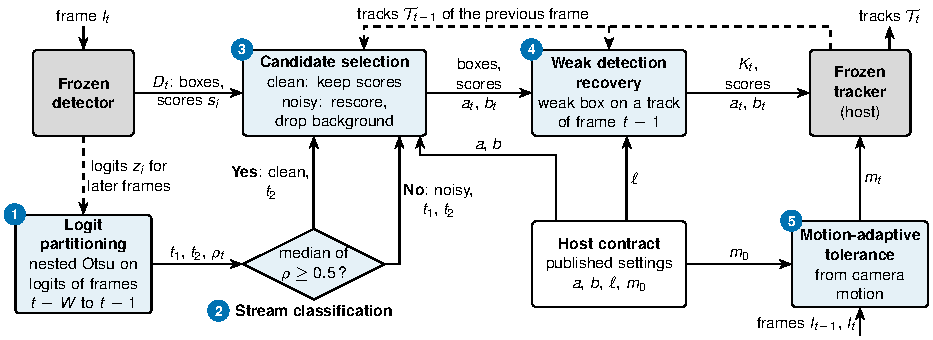
\includegraphics{Fig1.pdf}
\caption{\scl{} between a frozen detector and a frozen tracker (the host), for frame $t$. Arrows are
labelled with the data they carry; dashed arrows carry data from earlier frames. The diamond (Step 2)
is a decision: clean (Yes) if the median of $\rho$ is at least 0.5, noisy (No) otherwise. Steps 1--5:
Sects.~\ref{sec:calib}--\ref{sec:motion}; host contract: Sect.~\ref{sec:contract}; symbols:
Table~\ref{tab:symbols}}
\label{fig:arch}
\end{figure*}

\emph{Score calibration and adaptive inference.} Detector families such as YOLOX, YOLOv8, and
RT-DETR give different score distributions, and calibration methods learn a mapping from labelled
data \cite{kuppers2020detcalib}. Otsu's method picks, without labels, the threshold that best splits a
histogram into two groups \cite{goh2018otsu}; \scl{} applies it to the logits of recent scores. Dynamic
networks learn their settings for each model \cite{han2022dynamic}, and our earlier controller,
AC-MOT (submitted), sets the detector operating point from image and track cues. \scl{} instead
reads the scores and acts on the tracker's input and thresholds.
% --- sections/03_method
\section{Proposed SCL Framework}\label{sec:method}

\scl{} is a lightweight, rule-based layer operating between a frozen detector and tracker (the
host) without modifying their underlying algorithms. Fig.~\ref{fig:arch} illustrates the five
processing steps of \scl{} for frame $t$. First, Otsu-based logit partitioning (Step~1) divides
recent detection scores into background, uncertain, and confident groups. Next, detection stream
classification (Step~2) determines whether the score distribution is clean or noisy based on
historical confidence statistics. Mode-adaptive candidate selection (Step~3) then retains,
removes, or remaps detection scores and adjusts the tracker's confidence thresholds according to
the operating mode. Track-guided weak detection recovery (Step~4) allows eligible low-confidence
detections to support track continuity. Finally, camera motion-adaptive matching tolerance
(Step~5) adjusts the association criterion according to estimated camera motion. The host
contract provides the tracker's published parameters, while the tracker performs its original
association and track-management operations unchanged.

Table~\ref{tab:symbols} lists every symbol in plain words, with its value in the clean stream of
Fig.~\ref{fig:groups}a, which the subsections below follow from input to output.

% --- tables/tab_symbols
\begin{table*}[!tb]
\caption{The symbols of Sect.~\ref{sec:method} in plain words. Example: the value in the clean
stream of Fig.~\ref{fig:groups}a (MOT17-02, frame 101, ByteTrack in its official setting), as
recorded by the frozen \scl{}; e.g.: a worked example from the text.}
\label{tab:symbols}
\centering\footnotesize
\setlength{\tabcolsep}{3pt}
\begin{tabular}{@{}l>{\raggedright\arraybackslash}p{97mm}>{\raggedright\arraybackslash}p{40mm}@{}}
\toprule
Symbol & Meaning & Example\\
\midrule
$s_i$, $z_i$ & detector score of candidate $i$, between 0 and 1, and its logit, Eq.~\eqref{eq:logit} & e.g.\ 0.9 and $\log 9=2.2$\\
$W$, $Z_t^W$ & number of past frames whose logits are pooled; the logits of frames $t-W$ to $t-1$ & 10; 916 logits\\
$t_1$, $t_2$ & first split (background lies below it); second split (confident lies above it) & $-0.78$ (0.32); 0.95 (0.72)\\
$\rho_t$ & share of confident candidates in the foreground, Eq.~\eqref{eq:rho} & $175/263=0.67$\\
median $\rho$ & median of $\rho$ over the stream so far; clean if $\ge0.5$ & 0.63: clean\\
$a$, $b$, $\ell$ & the tracker's published scores to match a track and to start one, and the lowest score it uses & 0.6, 0.7, 0.1\\
$m_0$ & the tracker's matching tolerance: 1 minus the smallest IoU that matches & 0.8 (IoU $\ge0.2$)\\
$a_t$, $b_t$, $m_t$ & the thresholds and tolerance \scl{} passes for frame $t$, Eqs.~\eqref{eq:clean} and~\eqref{eq:motion} & 0.6, 0.7 (kept); 0.8\\
$u_i$, $\tilde{s}_i$ & rank of $s_i$ among stored scores; the new score of the noisy mode, Eq.~\eqref{eq:remap} & e.g.\ $u_i=0.8\to\tilde{s}_i=0.9$\\
$\mathcal{T}_{t-1}$, $K_t$ & the tracks of the previous frame; the candidates passed to the tracker & --\\
$g_t$, $r_t$ & camera shift between two frames; its ratio to the usual shift & e.g.\ $r_t=2$\\
\bottomrule
\end{tabular}
\end{table*}

\subsection{Inputs and outputs of SCL}\label{sec:problem}
In each frame $t$, the detector gives candidates $D_t=\{(\mathbf{x}_i,s_i,c_i)\}$, each with a box
$\mathbf{x}_i$, a score $s_i\in(0,1)$, and a class $c_i$. The layer works on the logit
\begin{equation}
z_i=\log\frac{s_i}{1-s_i},
\label{eq:logit}
\end{equation}
which keeps the order of the scores (0.5 gives $z_i=0$, 0.9 gives $\log9=2.2$, and 0.1 gives $-2.2$)
and spreads out the regions near 0 and 1, where detector scores crowd; the logistic function
$\sigma(z)=1/(1+e^{-z})$ maps a logit back to a score. The host gives its contract $h=(a,b,\ell,m_0)$:
the score $a$ needed to match a track, the score $b$ needed to start one, the lowest score $\ell$ it
uses, and its matching tolerance $m_0$, one minus the smallest intersection over union (IoU) that
counts as a match. A single-stage tracker has $\ell=\min(a,b)$, a two-stage tracker $\ell<\min(a,b)$.
For ByteTrack in its official setting, $a=0.6$, $b=0.7$, $\ell=0.1$, and $m_0=0.8$
(Table~\ref{tab:contracts}). In every frame the layer returns
\begin{equation}
\left(K_t,\tilde{s},a_t,b_t,m_t\right)=
\mathcal{L}\left(Z_{<t},D_t,\mathcal{T}_{t-1},g_t;\,h\right):
\label{eq:layer}
\end{equation}
the candidates $K_t$, their scores, and the thresholds and tolerance for the tracker, from the logits
$Z_{<t}$ of earlier frames, the tracks $\mathcal{T}_{t-1}$, and the camera motion $g_t$ between frames
$I_{t-1}$ and $I_t$; no future frame is used.

% --- tables/tab1_contracts
\begin{table*}[!t]
\caption{Host contracts: the four published settings $(a,b,\ell,m_0)$ of each tracker that \scl{}
reads (Sect.~\ref{sec:problem}), and where each value comes from; $\theta$: the published IoU
threshold, $m_0=1-\theta$.}
\label{tab:contracts}
\centering\footnotesize
\setlength{\tabcolsep}{4pt}
\begin{tabular}{@{}llcccc>{\raggedright\arraybackslash}p{84mm}@{}}
\toprule
Tracker (setting) & Type & $a$ & $b$ & $\ell$ & $m_0$ & Published settings behind the values\\
\midrule
ByteTrack (official) & two-stage & 0.6 & 0.7 & 0.1 & 0.8 & track\_thresh 0.6; new tracks $+$0.1; second step from 0.1; match\_thresh 0.8\\
ByteTrack (library) & two-stage & 0.25 & 0.25 & 0.1 & 0.8 & Ultralytics bytetrack.yaml: high 0.25, new 0.25, low 0.1, match 0.8\\
BoT-SORT (library) & two-stage & 0.25 & 0.25 & 0.1 & 0.8 & Ultralytics botsort.yaml: the same four values\\
SparseTrack & two-stage & 0.6 & 0.7 & 0.1 & 0.85 & track\_thresh 0.6; new tracks $+$0.1; second step from 0.1; match\_thresh 0.85\\
BoostTrack & two-stage & 0.6 & 0.6 & 0.1 & 0.7 & det\_thresh 0.6; every detection from 0.1 can be boosted; $\theta=0.3$\\
Hybrid-SORT & two-stage & 0.6 & 0.6 & 0.1 & 0.75 & det\_thresh 0.6; low-score step from 0.1; $\theta=0.25$\\
OC-SORT & single-stage & 0.6 & 0.6 & 0.6 & 0.7 & det\_thresh 0.6, no low-score step; $\theta=0.3$\\
PD-SORT & single-stage & 0.6 & 0.6 & 0.6 & 0.7 & det\_thresh 0.6, no low-score step; $\theta=0.3$\\
\bottomrule
\end{tabular}
\end{table*}

\subsection{Otsu-Based Logit Partitioning and Confidence Estimation}\label{sec:calib}
\emph{Step 1 in Fig.~\ref{fig:arch}. Input:} the logits $Z_t^W$ of the candidates of the last $W=10$
frames. \emph{Output:} the splits $t_1$, $t_2$ and the confident share $\rho_t$.

The logits are split twice with Otsu's method \cite{goh2018otsu}, which picks from the data alone the
threshold that best separates two groups: $t_1$ separates background (low logits) from foreground,
and $t_2$, found on the foreground only, divides it into uncertain and confident candidates. The
share of confident candidates in the foreground,
\begin{equation}
\rho_t=\frac{\left|\{z\in Z_t^W: z\ge t_2\}\right|}{\left|\{z\in Z_t^W: z\ge t_1\}\right|},
\label{eq:rho}
\end{equation}
describes the shape of the score distribution. In the clean stream of
Fig.~\ref{fig:groups}a, the window holds 916 candidates: 653 below $t_1=-0.78$ (score 0.32), 88
between the splits, and 175 above $t_2=0.95$ (score 0.72), so $\rho_t=175/(88+175)=0.67$; in the
noisy stream of Fig.~\ref{fig:groups}b, 1,037 are background, 99 uncertain, and 83 confident, so
$\rho_t=83/(99+83)=0.46$. As clutter usually gives more candidates than objects do, a window with
fewer candidates below $t_1$ than above it counts as clean, $\rho_t=1$ (background check), which does
not apply in Fig.~\ref{fig:groups}.

\begin{figure}[t]
\centering
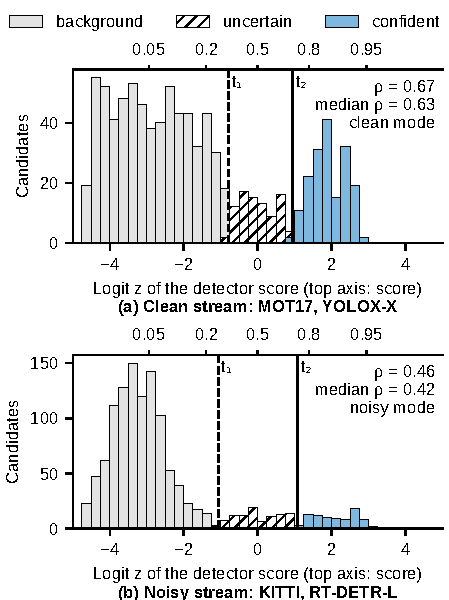
\includegraphics{Fig2.pdf}
\caption{What \scl{} sees before its decision for frame 101: the logits of the candidates of the last
10 frames (top axis: the same position as a score). Dashed line: $t_1$; solid line: $t_2$; light gray:
background; hatched: uncertain; blue: confident. (a) MOT17 sequence MOT17-02, YOLOX-X, ByteTrack
(official): median $\rho=0.63\ge0.5$, clean. (b) KITTI sequence 0001, RT-DETR-L, ByteTrack (library):
median $\rho=0.42<0.5$, noisy. Values recorded by the frozen \scl{}}
\label{fig:groups}
\end{figure}

\subsection{Median-Based Detection Stream Classification}\label{sec:regimes}
\emph{Step 2 in Fig.~\ref{fig:arch}. Input:} the values $\rho$ of all frames so far. \emph{Output:}
the mode of frame $t$.

The mode describes the distribution of the scores, not whether a single detection is correct: the
stream is clean at frame $t$ if the median of all $\rho$ values so far is at least one half, a
majority rule, and noisy otherwise; before the first valid split it is cold. In
Fig.~\ref{fig:groups}a, frames 2 to 101 give a median of 0.63, so frame 101 is clean; in
Fig.~\ref{fig:groups}b the median is 0.42, so it is noisy. The whole-stream median keeps the mode
stable against a few frames of blur or occlusion, while the groups, and in the clean mode the
thresholds of Step~3, follow a new score scale within $W$ frames.

\subsection{Mode-Adaptive Detection Candidate Selection and Threshold Adjustment}\label{sec:choice}
\emph{Step 3 in Fig.~\ref{fig:arch}. Input:} $D_t$, the mode, $t_1$, $t_2$, the thresholds $a$, $b$,
and the tracks $\mathcal{T}_{t-1}$. \emph{Output:} the kept boxes, their scores, and the thresholds
$a_t$, $b_t$.

\emph{Cold and clean modes.} The tracker keeps its own scores, and only cross-class duplicates are
removed. In the clean mode, a threshold that would reject the confident group is lowered to the
score $\sigma(t_2)$ at which that group begins:
\begin{equation}
a_t=\min\!\left(a,\sigma(t_2)\right),\qquad b_t=\min\!\left(b,\sigma(t_2)\right).
\label{eq:clean}
\end{equation}
In Fig.~\ref{fig:groups}a, $\sigma(t_2)=0.72$ is above both $a=0.6$ and $b=0.7$, so the published
thresholds are kept and the output equals that of the host alone (Sect.~\ref{sec:results}). When the
scores are halved, no score is above 0.5 and ByteTrack in its official setting never starts a track;
$\sigma(t_2)$ falls with the scores below 0.5, Eq.~\eqref{eq:clean} lowers both thresholds to it, and
the confident candidates reach the tracker again.

\emph{Noisy mode.} Background candidates ($z<t_1$) are dropped. Each remaining score is replaced by
its mid-rank $u_i\in(0,1)$ among the scores of a remap memory, which stores the scores kept in the
first frame and in every 10th frame, the last 20 of them (equal scores count half):
\begin{equation}
\tilde{s}_i=
\begin{cases}
0.5+0.5\,u_i, & z_i\ge t_2,\\
0.1+0.4\,u_i, & t_1\le z_i<t_2,
\end{cases}
\label{eq:remap}
\end{equation}
and both thresholds are set to $a_t=b_t=0.5$. A confident candidate with $u_i=0.8$ gets
$0.5+0.5\cdot0.8=0.9$ and may start and continue tracks; an uncertain one with $u_i=0.3$ gets
$0.1+0.4\cdot0.3=0.22$ and may only continue tracks through a tracker's low-score step. A weaker
candidate that overlaps a stronger one with IoU above one half is removed, unless a different track of
the previous frame claims it, which keeps people who stand close together in a crowd.

\emph{Score remapping is not probability calibration.} Calibration learns from labelled data the
probability that a detection is correct \cite{kuppers2020detcalib}. The remap needs no labels: it
keeps the order of the scores within each group and places the groups in fixed ranges, so that the
tracker's own thresholds read the layer's decision (above 0.5: ``may start a track''; 0.1 to 0.5:
``may only continue one''), and it is unchanged by any order-preserving change of the scores.

\subsection{Track-Guided Weak Detection Recovery}\label{sec:rescue}
\emph{Step 4 in Fig.~\ref{fig:arch}. Input:} the output of Step~3, the tracks $\mathcal{T}_{t-1}$,
and $\ell$. \emph{Output:} $K_t$, their scores, and $a_t$, $b_t$ for the tracker.

A track can be lost when its object gets low scores for a few frames, above all in a single-stage
tracker, which has no low-score step. The rescue passes such a candidate, with its score raised just
above the lowest threshold of the frame ($\ell$ for a two-stage tracker, the lower of $a_t$ and $b_t$
for a single-stage one), when it is in the foreground (or, for a single-stage tracker, when there is
no background group), overlaps a track of the previous frame with IoU of at least one half, no other
usable candidate covers that track, and the tracker could not see it otherwise. For ByteTrack in its
official setting, a rescued candidate gets $0.101$ and enters its low-score step; for OC-SORT in a
noisy frame it gets $0.501$. The tracker itself still decides, with its own matching, whether and to
which track the box is assigned.

\subsection{Camera Motion-Adaptive Matching Tolerance}\label{sec:motion}
\emph{Step 5 in Fig.~\ref{fig:arch}. Input:} the frames $I_{t-1}$, $I_t$ and the tolerance $m_0$.
\emph{Output:} the tolerance $m_t$ of frame $t$.

In noisy frames, the matching tolerance grows with camera motion, which moves boxes far from their
tracks; otherwise $m_t=m_0$. The motion $g_t$ is the shift between consecutive grayscale
frames at quarter resolution, found by phase correlation \cite{tong2019fourier}, and $r_t$ is its
ratio to its median over the last 100 frames ($r_t=1$ during a warm-up of 5 frames or if this median
is zero):
\begin{equation}
m_t=\min\!\left(0.95,\;1-\frac{1-m_0}{\max(1,r_t)}\right).
\label{eq:motion}
\end{equation}
With $m_0=0.8$, a match needs an IoU of at least 0.2; if the camera moves twice as much as usual
($r_t=2$), then $m_t=\min(0.95,\,1-0.2/2)=0.9$, and an IoU of 0.1 is enough. The cap 0.95 keeps a
smallest overlap of 0.05.

\subsection{SCL Integration with Existing Trackers}\label{sec:contract}
Each contract value in Table~\ref{tab:contracts} comes from the tracker's published configuration;
none is fitted. For each tracker family, a small adapter writes the layer's outputs into the
tracker's existing parameters and calls its own update, so the authors' matching, motion model,
track management, and post-processing run unchanged.


\begin{table}[!tb]
\caption{The fixed values of \scl{}, their settings, and their sources; the same values are used for every tracker, detector, and dataset.}
\label{tab:constants}
\centering\footnotesize
\setlength{\tabcolsep}{3pt}
\begin{tabular}{@{}>{\raggedright\arraybackslash}p{23mm}>{\raggedright\arraybackslash}p{29.5mm}>{\raggedright\arraybackslash}p{19mm}@{}}
\toprule
Value & Setting & Source\\
\midrule
Window $W$ & 10 frames & design choice\\
Mode rule & clean if median $\rho\ge0.5$ & majority rule\\
Background check & $\rho=1$ if fewer below $t_1$ & no background\\
Noisy score ranges & $[0.5,1)$, $[0.1,0.5)$ & common values\\
Noisy $a_t$, $b_t$ & 0.5 & common value\\
Remap memory & 20 frames, every 10th & design choice\\
Duplicate, rescue IoU & 0.5 & MOT evaluation\\
Rescued score & lowest threshold $+\,0.001$ & just above it\\
Motion cue & phase correlation, $\tfrac{1}{4}$ size & standard \cite{tong2019fourier}\\
Motion history & 100 frames, warm-up 5 & design choice\\
Tolerance cap & 0.95 & overlap $\ge0.05$\\
\bottomrule
\end{tabular}
\end{table}

\subsection{Fixed SCL Parameters}\label{sec:constants}
Table~\ref{tab:constants} lists all values of \scl{}. They were fixed before the external
evaluation, and none was chosen by searching over a range of values: they are standard values (the
IoU of 0.5 of MOT evaluation and the common thresholds 0.5 and 0.1), definitions, or design choices
kept fixed in all development stages. Algorithm~\ref{alg:layer} gives Steps 1--5 for one frame.

\begin{algorithm}[t]
\caption{\scl{} for frame $t$; the comments name the steps of Fig.~\ref{fig:arch}. The window
holds the logits of frames $t-W$ to $t-1$, so the decision for frame $t$ uses no future frame.}\label{alg:layer}
\begin{algorithmic}[1]
\Require candidates $D_t$, tracks $\mathcal{T}_{t-1}$, motion cue $g_t$, contract $(a,b,\ell,m_0)$, constants of Table~\ref{tab:constants}
\Ensure candidates $K_t$, scores $\tilde{s}$, thresholds $a_t,b_t$, tolerance $m_t$
\State $z_i\gets$ logit of $s_i$ for all $i$ \Comment{Eq.~\eqref{eq:logit}}
\If{no valid split exists} \Comment{e.g., first frame}
  \State mode $\gets$ cold; $(a_t,b_t)\gets(a,b)$
\Else
  \State $(t_1,t_2)\gets$ nested Otsu on the window \Comment{Step 1}
  \State $\rho_t\gets$ Eq.~\eqref{eq:rho} with the background check
  \State mode $\gets$ clean if $\mathrm{median}(\rho)\ge0.5$, else noisy \Comment{Step 2}
\EndIf
\If{mode is cold or clean} \Comment{Step 3}
  \State remove cross-class duplicates; keep raw scores
  \State if clean, set $(a_t,b_t)$ by Eq.~\eqref{eq:clean}
\Else \Comment{noisy mode}
  \State remove duplicates with track context
  \State drop $z<t_1$; remap by Eq.~\eqref{eq:remap}; $a_t,b_t\gets0.5$
\EndIf
\State rescue continuations (not cold) \Comment{Step 4}
\State $m_t\gets$ Eq.~\eqref{eq:motion} if noisy, else $m_0$ \Comment{Step 5}
\State pass $K_t$, $\tilde{s}$, $a_t$, $b_t$, $m_t$ to the tracker
\State update the window (logits left after duplicate removal), the motion history ($g_t$), and the stored tracks after the tracker update
\end{algorithmic}
\end{algorithm}
% --- sections/04_development
\section{SCL Development and Refinement}\label{sec:development}

This section presents the development and refinement of \scl{} using the development data
described in Sect.~\ref{sec:data}. Section~\ref{sec:prior} introduces the initial always-on banding
(\aob{}) design and discusses its limitations (Table~\ref{tab:prior}). Section~\ref{sec:steps}
describes the incremental improvements that addressed these limitations, supported by the
experimental comparisons in Table~\ref{tab:ablation}. Finally, Sect.~\ref{sec:freeze} explains the
configuration freezing and validation procedures performed before external evaluation to ensure
reproducibility and prevent changes based on subsequent results.

% --- tables/tab_prior
\begin{table*}[!t]
\caption{MOT17 val-half, published YOLOX-X detections: the earlier design \aob{} and the final \scl{}, each added to the same strong tracker (Host). Change: the run with the layer minus Host, with its 95\% bootstrap interval; bold: the interval does not include zero (a reliable change).}
\label{tab:prior}
\centering\footnotesize
\setlength{\tabcolsep}{6pt}
\begin{tabular}{@{}lrrlrl@{}}
\toprule
Metric & Host & Host+\aob{} & \aob{} change [95\% CI] & Host+\scl{} & \scl{} change [95\% CI]\\
\midrule
\multicolumn{6}{@{}l}{\textit{SparseTrack} \cite{liu2025sparsetrack}}\\
\quad HOTA$\uparrow$ & 68.88 & 64.72 & {\boldmath $-4.15$ [$-5.54$, $-1.66$]} & 68.93 & $+0.06$ [$-0.01$, $+0.25$]\\
\quad MOTA$\uparrow$ & 77.85 & 71.71 & {\boldmath $-6.14$ [$-8.10$, $-2.74$]} & 77.93 & $+0.08$ [$-0.03$, $+0.30$]\\
\quad IDF1$\uparrow$ & 81.97 & 77.49 & {\boldmath $-4.49$ [$-6.19$, $-1.96$]} & 82.13 & $+0.16$ [$-0.02$, $+0.70$]\\
\multicolumn{6}{@{}l}{\textit{BoostTrack, online} \cite{stanojevic2024boosttrack}}\\
\quad HOTA$\uparrow$ & 68.49 & 62.61 & {\boldmath $-5.89$ [$-7.76$, $-2.87$]} & 68.49 & 0 (identical)\\
\quad MOTA$\uparrow$ & 75.50 & 66.64 & {\boldmath $-8.87$ [$-12.37$, $-7.14$]} & 75.50 & 0 (identical)\\
\quad IDF1$\uparrow$ & 81.41 & 75.19 & {\boldmath $-6.22$ [$-9.33$, $-2.85$]} & 81.41 & 0 (identical)\\
\multicolumn{6}{@{}l}{\textit{BoostTrack, with GBI} \cite{stanojevic2024boosttrack}}\\
\quad HOTA$\uparrow$ & 71.73 & 66.35 & {\boldmath $-5.37$ [$-7.30$, $-2.75$]} & 71.73 & 0 (identical)\\
\quad MOTA$\uparrow$ & 81.03 & 72.30 & {\boldmath $-8.73$ [$-12.59$, $-6.50$]} & 81.03 & 0 (identical)\\
\quad IDF1$\uparrow$ & 84.16 & 78.51 & {\boldmath $-5.65$ [$-8.96$, $-2.77$]} & 84.16 & 0 (identical)\\
\bottomrule
\end{tabular}
\end{table*}
% --- tables/tab6_ablation
\begin{table*}[!tp]
\caption{How \scl{} was built from \aob{} on development data. Each row adds one change to the row above; Effect gives the HOTA (\%) before and after that change (``A to B'') or compared with the tracker alone (host). The number in parentheses after ByteTrack and OC-SORT is the lowest emitted detector score.}
\label{tab:ablation}
\centering\footnotesize
\setlength{\tabcolsep}{4pt}
\begin{tabular}{@{}>{\raggedright\arraybackslash}p{30mm}>{\raggedright\arraybackslash}p{48mm}>{\raggedright\arraybackslash}p{74mm}@{}}
\toprule
Step & Change & Effect\\
\midrule
\aob{} emulated & always-noisy bands, overlap deduplication, rank remap & ByteTrack (0.1) 56.41 vs host 67.70; OC-SORT (0.1) 45.72 vs 66.44\\
+ mode gate & mode statistic, host-anchored clean mode, crowd-safe duplicates & SparseTrack 64.72 to 68.93 (host 68.88); BoostTrack 62.61 to 68.37 (host 68.49)\\
+ whole-stream mode & mode from all past frames & ByteTrack (0.1) 67.561 to 67.702; OC-SORT (0.1) 65.697 to 66.071\\
+ continuation rescue & foreground track-consistent rescue & OC-SORT (0.01) 66.405 to 66.619; OC-SORT (0.1) 66.071 to 66.469\\
+ background check = \scl{} & no background mode gives no evidence against the host & ByteTrack/BoostTrack (0.1) identical to host; OC-SORT 67.041 (0.01), 66.907 (0.1)\\
\bottomrule
\end{tabular}
\end{table*}
\subsection{Initial Design and Limitations}\label{sec:prior}
The earlier design \aob{} computed the same nested Otsu groups but treated every stream as noisy:
in every frame it applied the groups, removed every weaker candidate that overlapped a stronger one
with IoU above one half, and rescored all candidates by rank. On strong MOT17 trackers
(Table~\ref{tab:prior}), \aob{} lowered HOTA by 4.15 to 5.89 points, as the overlap rule deleted
people hidden behind others in crowds and its thresholds were stricter than the trackers' own; with
the same trackers, \scl{} changed HOTA by $+0.06$ for SparseTrack and left BoostTrack, online and with
its gap-filling post-processing (GBI), identical to the host. The next steps therefore let the layer
decide from the scores whether to act at all.

\subsection{Incremental Design Improvements}\label{sec:steps}
Each step was compared with the step before it (Table~\ref{tab:ablation}). The \emph{mode gate}
added the mode check, the clean mode that keeps the tracker's scores and thresholds, and the
crowd-safe duplicate rule, and restored SparseTrack and BoostTrack to the accuracy of their hosts.
The \emph{whole-stream mode} removed mode changes in the middle of streams and raised ByteTrack and
OC-SORT, and the \emph{continuation rescue} added 0.2 to 0.4 points for OC-SORT. The
\emph{background check} completed \scl{}: ByteTrack and BoostTrack returned to output identical to
the host, and OC-SORT rose to 67.04 and 66.91 at the two floors.

\subsection{Configuration Freezing and Validation}\label{sec:freeze}
The final configuration was frozen before any external test as a version-control tag, with a lock
file holding a cryptographic hash of the layer, its configuration, and the evaluation scripts;
sixty-one automated tests check, among others, that the layer uses no future data and passes clean
streams unchanged. All results of Sect.~\ref{sec:results} come from this frozen configuration; the
comparisons, ablation, and sensitivity analysis used run-time options of the evaluation scripts and
changed none of its values.
% --- sections/05_results
\section{Experimental Results and Evaluation}\label{sec:results}

This section evaluates the effectiveness and generalization of \scl{} against the host trackers
using identical detections and published tracker configurations. Section~\ref{sec:tracker}
examines tracking performance across different trackers on MOT17, while Sect.~\ref{sec:detector}
evaluates detector--tracker compatibility on KITTI. Section~\ref{sec:shift} investigates robustness
to detection confidence-score shifts, and Sect.~\ref{sec:baselines} compares \scl{} with adaptive
thresholding methods. Section~\ref{sec:ablation} presents component ablation and parameter
sensitivity analyses. Finally, Sects.~\ref{sec:external} and~\ref{sec:visdrone} assess
generalization to previously unseen trackers and the held-out UAVDT dataset, respectively. In all
comparisons, the baseline is the host tracker operating without \scl{}, and Fig.~\ref{fig:forest}
summarizes the HOTA differences across the evaluated configurations.

\emph{How to read the result tables.} Each row gives one metric of the tracker alone (Host) and
with \scl{} (Host+\scl{}), and Change with its 95\% interval (Sect.~\ref{sec:metrics}); a bold change
is reliable, and ``identical'' means an unchanged output. For example, in Table~\ref{tab:mot17},
OC-SORT at floor 0.01 has a MOTA of 74.67 alone and 75.94 with \scl{}: the change is $+1.27$ points,
and its interval $[+0.17,+3.01]$ lies above zero, so the gain is reliable.
Values are rounded separately, so Host+\scl{} minus Host can differ from Change in the last digit.

\begin{figure}[!t]
\centering
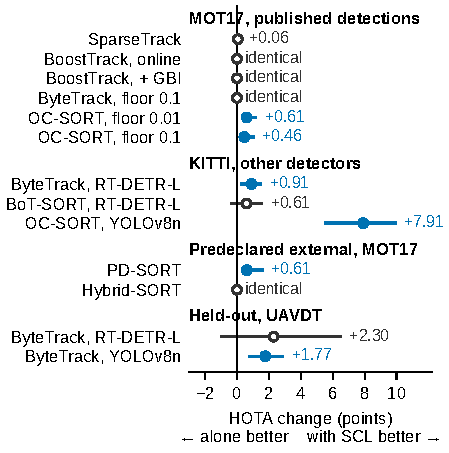
\includegraphics{Fig3.pdf}
\caption{HOTA change with \scl{} (tracker with \scl{} minus tracker alone, in points) for the
tested trackers and detectors. Dot and number: the change; line: its 95\% bootstrap interval; right
of zero, \scl{} is better. Filled dot: a reliable gain; open dot: no reliable change or identical
output}
\label{fig:forest}
\end{figure}

\subsection{Performance Across Trackers on MOT17}\label{sec:tracker}
Table~\ref{tab:mot17} shows the development trackers on MOT17 val-half. The two-stage trackers with
well-matched detections kept the accuracy of their hosts: BoostTrack, online and with GBI, and
ByteTrack at floor 0.1 gave exactly the same output, and SparseTrack rose by 0.06 HOTA points
through the self-limiting clean mode. The single-stage OC-SORT improved at both floors (HOTA from
66.43 to 67.04 and from 66.44 to 66.91, MOTA $+1.27$ and $+1.26$), with fewer identity switches and
higher HOTA on 7 of 7 sequences, through the continuation rescue.

% --- tables/tab3_mot17
\begin{table}[!tb]
\caption{MOT17 val-half, published YOLOX-X detections: each development tracker alone (Host) and with \scl{} (Host+\scl{}). Change: Host+\scl{} minus Host, with its 95\% bootstrap interval; bold: a reliable change. Paper: the value reported by the tracker's authors (--: not reported). Floor: the lowest emitted detector score.}
\label{tab:mot17}
\centering\footnotesize
\setlength{\tabcolsep}{2.5pt}
\begin{tabular}{@{}lrrrl@{}}
\toprule
Metric & Paper & Host & \begin{tabular}[b]{@{}r@{}}Host\\+\scl{}\end{tabular} & Change [95\% CI]\\
\midrule
\multicolumn{5}{@{}l}{\textit{SparseTrack} \cite{liu2025sparsetrack}}\\
\quad HOTA$\uparrow$ & 69.2 & 68.88 & 68.93 & $+0.06$ [$-0.01$, $+0.25$]\\
\quad MOTA$\uparrow$ & 76.8 & 77.85 & 77.93 & $+0.08$ [$-0.03$, $+0.30$]\\
\quad IDF1$\uparrow$ & 81.4 & 81.97 & 82.13 & $+0.16$ [$-0.02$, $+0.70$]\\
\multicolumn{5}{@{}l}{\textit{BoostTrack, online} \cite{stanojevic2024boosttrack}}\\
\quad HOTA$\uparrow$ & 68.37 & 68.49 & 68.49 & 0 (identical)\\
\quad MOTA$\uparrow$ & 75.56 & 75.50 & 75.50 & 0 (identical)\\
\quad IDF1$\uparrow$ & 81.35 & 81.41 & 81.41 & 0 (identical)\\
\quad IDS$\downarrow$ & 118 & 113 & 113 & 0 (identical)\\
\multicolumn{5}{@{}l}{\textit{BoostTrack, + GBI} \cite{stanojevic2024boosttrack}}\\
\quad HOTA$\uparrow$ & 71.33 & 71.73 & 71.73 & 0 (identical)\\
\quad MOTA$\uparrow$ & 80.55 & 81.03 & 81.03 & 0 (identical)\\
\quad IDF1$\uparrow$ & 83.84 & 84.16 & 84.16 & 0 (identical)\\
\quad IDS$\downarrow$ & 106 & 97 & 97 & 0 (identical)\\
\multicolumn{5}{@{}l}{\textit{ByteTrack, floor 0.1} \cite{zhang2022bytetrack}}\\
\quad HOTA$\uparrow$ & -- & 67.70 & 67.70 & 0 (identical)\\
\quad MOTA$\uparrow$ & 76.6 & 77.60 & 77.60 & 0 (identical)\\
\quad IDF1$\uparrow$ & 79.3 & 79.47 & 79.47 & 0 (identical)\\
\quad IDS$\downarrow$ & -- & 214 & 214 & 0 (identical)\\
\multicolumn{5}{@{}l}{\textit{OC-SORT, floor 0.01} \cite{cao2023ocsort}}\\
\quad HOTA$\uparrow$ & 66.5 & 66.43 & 67.04 & {\boldmath $+0.61$ [$+0.36$, $+1.24$]}\\
\quad MOTA$\uparrow$ & 74.9 & 74.67 & 75.94 & {\boldmath $+1.27$ [$+0.17$, $+3.01$]}\\
\quad IDF1$\uparrow$ & 77.7 & 78.05 & 78.71 & $+0.66$ [$-0.25$, $+1.60$]\\
\quad IDS$\downarrow$ & -- & 211 & 203 & {\boldmath $-8$ [$-15$, $-2$]}\\
\multicolumn{5}{@{}l}{\textit{OC-SORT, floor 0.1} \cite{cao2023ocsort}}\\
\quad HOTA$\uparrow$ & 66.5 & 66.44 & 66.91 & {\boldmath $+0.46$ [$+0.27$, $+1.09$]}\\
\quad MOTA$\uparrow$ & 74.9 & 74.67 & 75.93 & {\boldmath $+1.26$ [$+0.37$, $+3.34$]}\\
\quad IDF1$\uparrow$ & 77.7 & 78.05 & 78.33 & {\boldmath $+0.287$ [$+0.003$, $+0.838$]}\\
\quad IDS$\downarrow$ & -- & 213 & 199 & $-14$ [$-38$, $+6$]\\
\bottomrule
\end{tabular}
\end{table}

\subsection{Cross-Detector Evaluation on KITTI}\label{sec:detector}
\begin{figure*}[t]
\centering
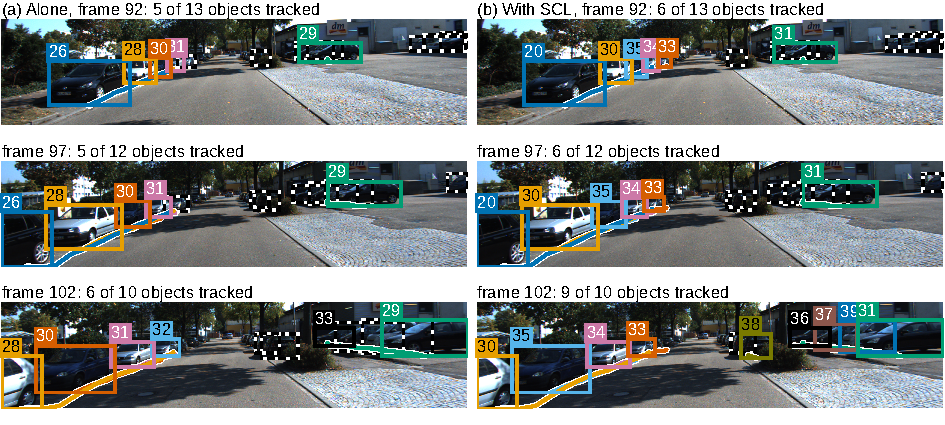
\includegraphics{Fig4.pdf}
\caption{KITTI sequence 0001 \cite{geiger2012kitti} tracked by OC-SORT with YOLOv8n at frames 92,
97, and 102 (rows): (a) the tracker alone; (b) with \scl{}. Each colour and number is one track; its
line shows the object's last 20 frames. Dashed boxes: labelled objects that no track follows. IDs
are numbered separately in each run. The sequence has the median HOTA gain of the 21 sequences, and frame 102 is
its first frame with the largest gain in tracked objects}
\label{fig:example}
\end{figure*}
Table~\ref{tab:kitti} shows what happens when the detector is replaced. With the noisy RT-DETR-L,
\scl{} raised ByteTrack by 5.98 MOTA, 3.87 IDF1, and 0.91 HOTA points and BoT-SORT by 7.86 MOTA,
3.10 IDF1, and 0.61 HOTA points, with 297 and 226 fewer identity switches. With YOLOv8n, OC-SORT
rose from 36.27 to 44.18 HOTA ($+7.91$ points, $[+5.47,+9.98]$), 9.40 MOTA points, and 9.60 IDF1
points, as its missed objects (FN) fell by 5,310. Fig.~\ref{fig:example} follows this cell over
three frames: each object keeps its ID, and at frame 102 OC-SORT alone tracked 6 of the 10 labelled
objects and with \scl{} 9.

% --- tables/tab4_kitti
\begin{table}[!tb]
\caption{KITTI tracking training with detectors the trackers were not tuned for (HOTA averaged over cars and pedestrians); columns as in Table~\ref{tab:mot17}. BoT-SORT leaves out sequence 0020 in both runs, because its code stops with a numerical error on it.}
\label{tab:kitti}
\centering\footnotesize
\setlength{\tabcolsep}{2.5pt}
\begin{tabular}{@{}lrrl@{}}
\toprule
Metric & Host & \begin{tabular}[b]{@{}r@{}}Host\\+\scl{}\end{tabular} & Change [95\% CI]\\
\midrule
\multicolumn{4}{@{}l}{\textit{ByteTrack} \cite{zhang2022bytetrack}\textit{, RT-DETR-L}}\\
\quad HOTA$\uparrow$ & 50.73 & 51.64 & {\boldmath $+0.91$ [$+0.22$, $+1.55$]}\\
\quad MOTA$\uparrow$ & 47.27 & 53.24 & {\boldmath $+5.98$ [$+1.16$, $+9.94$]}\\
\quad IDF1$\uparrow$ & 64.98 & 68.86 & {\boldmath $+3.87$ [$+1.67$, $+5.06$]}\\
\quad IDS$\downarrow$ & 686 & 389 & {\boldmath $-297$ [$-530$, $-122$]}\\
\multicolumn{4}{@{}l}{\textit{BoT-SORT} \cite{aharon2022botsort}\textit{, RT-DETR-L} (20 sequences)}\\
\quad HOTA$\uparrow$ & 53.91 & 54.52 & $+0.61$ [$-0.39$, $+1.61$]\\
\quad MOTA$\uparrow$ & 48.25 & 56.11 & {\boldmath $+7.86$ [$+2.21$, $+13.44$]}\\
\quad IDF1$\uparrow$ & 67.74 & 70.85 & {\boldmath $+3.10$ [$+1.00$, $+4.57$]}\\
\quad IDS$\downarrow$ & 476 & 250 & {\boldmath $-226$ [$-369$, $-120$]}\\
\multicolumn{4}{@{}l}{\textit{OC-SORT} \cite{cao2023ocsort}\textit{, YOLOv8n}}\\
\quad HOTA$\uparrow$ & 36.27 & 44.18 & {\boldmath $+7.91$ [$+5.47$, $+9.98$]}\\
\quad MOTA$\uparrow$ & 33.99 & 43.39 & {\boldmath $+9.40$ [$+1.10$, $+12.30$]}\\
\quad IDF1$\uparrow$ & 50.46 & 60.05 & {\boldmath $+9.60$ [$+5.61$, $+12.16$]}\\
\bottomrule
\end{tabular}
\end{table}
% --- tables/tab_shift
\begin{table}[!tb]
\caption{MOT17 val-half with the detector scores changed before the tracker, which keeps its published thresholds: $s^3$ cubes every score, $0.5\,s$ halves it, and $T=2$ and $T=0.5$ divide its logit by 2 or 0.5. HOTA of the tracker alone (Host) and with \scl{} (Host+\scl{}); 0.00: no object tracked; Change with its 95\% bootstrap interval; bold: a reliable change. Lowest emitted score 0.01 (BoostTrack 0.1).}
\label{tab:shift}
\centering\footnotesize
\setlength{\tabcolsep}{3pt}
\begin{tabular}{@{}lrrl@{}}
\toprule
 & \multicolumn{3}{c}{HOTA (\%)}\\
\cmidrule(l){2-4}
Score change & Host & \begin{tabular}[b]{@{}r@{}}Host\\+\scl{}\end{tabular} & Change [95\% CI]\\
\midrule
\multicolumn{4}{@{}l}{\textit{ByteTrack, official setting} \cite{zhang2022bytetrack}}\\
\quad $s^3$ & 60.92 & 65.81 & {\boldmath $+4.89$ [$+2.60$, $+13.69$]}\\
\quad $0.5\,s$ & 0.00 & 66.17 & {\boldmath $+66.17$ [$+49.32$, $+75.40$]}\\
\quad $T=2$ & 65.84 & 66.95 & {\boldmath $+1.11$ [$+0.35$, $+3.87$]}\\
\multicolumn{4}{@{}l}{\textit{OC-SORT} \cite{cao2023ocsort}}\\
\quad $s^3$ & 58.34 & 66.60 & {\boldmath $+8.26$ [$+5.86$, $+16.81$]}\\
\quad $0.5\,s$ & 0.00 & 66.72 & {\boldmath $+66.72$ [$+50.32$, $+75.56$]}\\
\quad $T=2$ & 65.99 & 67.22 & {\boldmath $+1.24$ [$+0.52$, $+3.42$]}\\
\quad $T=0.5$ & 66.61 & 67.06 & $+0.45$ [$-0.01$, $+0.97$]\\
\multicolumn{4}{@{}l}{\textit{BoostTrack, online} \cite{stanojevic2024boosttrack}}\\
\quad $s^3$ & 61.33 & 64.84 & {\boldmath $+3.51$ [$+0.85$, $+13.28$]}\\
\quad $T=2$ & 67.59 & 67.59 & 0 (identical)\\
\bottomrule
\end{tabular}
\end{table}
% --- tables/tab_baselines
\begin{table}[!tb]
\caption{KITTI tracking training: HOTA of the tracker alone (Host), of two adaptive baselines that set the tracker's thresholds in every frame to the first ($t_1$) or second ($t_2$) Otsu split of the logits of the last 10 frames, and of \scl{}. Halved: halved detector scores. \scl{} $-$ $t_2$: the gain over the stronger baseline, with its 95\% bootstrap interval below; bold: a reliable gain.}
\label{tab:baselines}
\centering\footnotesize
\setlength{\tabcolsep}{3pt}
\begin{tabular}{@{}lrrrrc@{}}
\toprule
Cell & Host & $t_1$ & $t_2$ & \scl{} & \scl{} $-$ $t_2$\\
\midrule
\twol{OC-SORT,}{YOLOv8n} & 36.27 & 39.97 & 41.09 & 44.18 & \cib{+3.09}{+2.00}{+4.03}\\
\addlinespace[3pt]
\begin{tabular}[c]{@{}l@{}}ByteTrack,\\RT-DETR-L,\\halved\end{tabular} & 49.50 & 49.58 & 49.50 & 51.79 & \cib{+2.29}{+0.28}{+4.96}\\
\addlinespace[3pt]
\begin{tabular}[c]{@{}l@{}}OC-SORT,\\YOLOv8n,\\halved\end{tabular} & 0.00 & 37.68 & 43.56 & 46.30 & \cib{+2.74}{+1.32}{+3.34}\\
\bottomrule
\end{tabular}
\end{table}
% --- tables/tab_act
\begin{table*}[!tp]
\caption{ACT \cite{act2026adaptive}, with its published parameters, and \scl{} on the same detections and tracker. (a) HOTA with each method, and \scl{} $-$ ACT in HOTA and IDF1 with its 95\% bootstrap interval. (b) MOTA and identity switches on UAVDT. A positive HOTA, IDF1, or MOTA difference and a negative IDS difference favour \scl{}; bold: a reliable difference. KITTI: HOTA averaged over cars and pedestrians; MOT17: val-half, the setting ACT was designed for; UAVDT: test split.}
\label{tab:act}
\centering\footnotesize
\setlength{\tabcolsep}{3pt}
{\textit{(a) HOTA and IDF1}}\par\smallskip
\begin{tabular}{@{}lllrrll@{}}
\toprule
Data & Detector & Tracker & ACT & \scl{} & \scl{} $-$ ACT, HOTA [95\% CI] & \scl{} $-$ ACT, IDF1 [95\% CI]\\
\midrule
KITTI, halved & RT-DETR-L & ByteTrack & 49.77 & 51.79 & {\boldmath $+2.01$ [$+0.01$, $+4.76$]} & $+1.70$ [$-1.13$, $+6.80$]\\
KITTI, halved & YOLOv8n & OC-SORT & 36.24 & 46.30 & {\boldmath $+10.06$ [$+6.88$, $+12.01$]} & {\boldmath $+12.03$ [$+6.85$, $+14.69$]}\\
\addlinespace[2pt]
MOT17, floor 0.01 & YOLOX-X & ByteTrack (official) & 67.46 & 67.68 & $+0.22$ [$-0.43$, $+0.88$] & $+0.57$ [$-0.68$, $+2.12$]\\
MOT17, floor 0.1 & YOLOX-X & ByteTrack (official) & 67.46 & 67.70 & $+0.23$ [$-0.40$, $+0.90$] & $+0.60$ [$-0.55$, $+2.10$]\\
\addlinespace[2pt]
UAVDT test & YOLOv8n & ByteTrack & 29.01 & 30.83 & {\boldmath $+1.82$ [$+0.65$, $+3.00$]} & {\boldmath $+4.00$ [$+1.85$, $+6.22$]}\\
UAVDT test & RT-DETR-L & ByteTrack & 40.14 & 42.37 & $+2.23$ [$-0.97$, $+6.32$] & $+5.35$ [$-0.03$, $+12.47$]\\
\bottomrule
\end{tabular}

\medskip
{\textit{(b) MOTA and identity switches on UAVDT (test split, ByteTrack)}}\par\smallskip
\begin{tabular}{@{}lrrlrrl@{}}
\toprule
 & \multicolumn{3}{c}{MOTA$\uparrow$} & \multicolumn{3}{c}{IDS$\downarrow$}\\
\cmidrule(lr){2-4}\cmidrule(l){5-7}
Detector & ACT & \scl{} & \scl{} $-$ ACT [95\% CI] & ACT & \scl{} & \scl{} $-$ ACT [95\% CI]\\
\midrule
YOLOv8n & 16.59 & 17.29 & $+0.71$ [$-1.42$, $+2.52$] & 578 & 393 & $-185$ [$-480$, $+13$]\\
RT-DETR-L & 5.34 & 27.99 & {\boldmath $+22.65$ [$+9.03$, $+47.21$]} & 873 & 455 & {\boldmath $-418$ [$-718$, $-123$]}\\
\bottomrule
\end{tabular}
\end{table*}
% --- tables/tab_compabl
\begin{table}[!tb]
\caption{What each part and each fixed value of \scl{} contributes on the three KITTI cells of Table~\ref{tab:baselines} (HOTA): (a) OC-SORT, YOLOv8n; (b) ByteTrack, RT-DETR-L, halved scores; (c) OC-SORT, YOLOv8n, halved scores. Middle: one part removed at a time, with the largest HOTA loss and its cell. Lower: one fixed value changed at a time (frozen value in brackets), with the largest HOTA change over the tested values and cells.}
\label{tab:compabl}
\centering\footnotesize
\setlength{\tabcolsep}{3pt}
\begin{tabular}{@{}lrc@{}}
\toprule
\multicolumn{3}{@{}l}{Frozen \scl{}, HOTA: (a) 44.18, (b) 51.79, (c) 46.30}\\
\midrule
Part removed & Largest loss & Cell\\
\midrule
Weak detection recovery & 3.35 & (a)\\
Noisy mode (always clean) & 2.44 & (c)\\
Remap (raw scores) & 1.67 & (b)\\
Motion tolerance & 0.14 & (c)\\
\midrule
Value changed (frozen) & Largest change & Tested\\
\midrule
Window $W$ (10 frames) & 0.56 & 5, 20\\
Mode median frames (all) & 0.36 & last 100, 300\\
Duplicate/recovery IoU (0.5) & 0.62 & 0.4, 0.6\\
Motion history (100 frames) & 0.09 & 50, 200\\
\bottomrule
\end{tabular}
\end{table}
% --- tables/tab_generalization
\begin{table}[!tb]
\caption{Generalization, each run once with the frozen \scl{}; columns as in Table~\ref{tab:mot17}. (a) The two external trackers, chosen before the run and not used during design (MOT17 val-half, the authors' detections); Paper: the authors' number (for PD-SORT, their released output); EXACT: Host within 0.2 HOTA of it; CLOSE: within 1.0. (b) The held-out UAVDT test split (20 drone videos, not used during design), ByteTrack with its published setting.}
\label{tab:external}
\centering\footnotesize
\setlength{\tabcolsep}{2.5pt}
\begin{tabular}{@{}lrrrl@{}}
\toprule
Metric & Paper & Host & \begin{tabular}[b]{@{}r@{}}Host\\+\scl{}\end{tabular} & Change [95\% CI]\\
\midrule
\multicolumn{5}{@{}l}{(a) \textit{PD-SORT} \cite{wang2025pdsort}\textit{, EXACT}}\\
\quad HOTA$\uparrow$ & 68.01 & 68.01 & 68.62 & {\boldmath $+0.61$ [$+0.27$, $+1.65$]}\\
\quad MOTA$\uparrow$ & 75.19 & 75.19 & 76.31 & {\boldmath $+1.13$ [$+0.27$, $+3.03$]}\\
\quad IDF1$\uparrow$ & 81.03 & 81.03 & 81.85 & {\boldmath $+0.82$ [$+0.43$, $+1.94$]}\\
\multicolumn{5}{@{}l}{\textit{Hybrid-SORT} \cite{yang2024hybridsort}\textit{, CLOSE}}\\
\quad HOTA$\uparrow$ & 67.1 & 66.70 & 66.70 & 0 (identical)\\
\quad MOTA$\uparrow$ & 75.8 & 75.52 & 75.52 & 0 (identical)\\
\quad IDF1$\uparrow$ & 78.0 & 77.56 & 77.56 & 0 (identical)\\
\quad IDS$\downarrow$ & -- & 259 & 259 & 0 (identical)\\
\midrule
\multicolumn{5}{@{}l}{(b) \textit{ByteTrack, RT-DETR-L} \cite{zhang2022bytetrack,zhao2024rtdetr}}\\
\quad HOTA$\uparrow$ &  & 40.07 & 42.37 & $+2.30$ [$-1.05$, $+6.55$]\\
\quad MOTA$\uparrow$ &  & 3.29 & 27.99 & {\boldmath $+24.70$ [$+10.06$, $+51.08$]}\\
\quad IDF1$\uparrow$ &  & 48.59 & 54.33 & {\boldmath $+5.74$ [$+0.13$, $+13.11$]}\\
\quad IDS$\downarrow$ &  & 1041 & 455 & {\boldmath $-586$ [$-951$, $-248$]}\\
\multicolumn{5}{@{}l}{\textit{ByteTrack, YOLOv8n} \cite{zhang2022bytetrack,jocher2023yolov8}}\\
\quad HOTA$\uparrow$ &  & 29.05 & 30.83 & {\boldmath $+1.77$ [$+0.70$, $+2.94$]}\\
\quad MOTA$\uparrow$ &  & 16.27 & 17.29 & $+1.02$ [$-1.06$, $+2.86$]\\
\quad IDF1$\uparrow$ &  & 34.52 & 38.49 & {\boldmath $+3.97$ [$+1.88$, $+6.17$]}\\
\quad IDS$\downarrow$ &  & 719 & 393 & {\boldmath $-326$ [$-691$, $-73$]}\\
\bottomrule
\end{tabular}
\end{table}

\subsection{Robustness to Detection Score Shifts}\label{sec:shift}
Table~\ref{tab:shift} shows the trackers under the four score transforms. Halving the scores
reduced ByteTrack (official setting) and OC-SORT to 0 HOTA; with the layer they reached 66.17 and
66.72. Cubing reduced them to 60.92 and 58.34, and the layer restored them to 65.81 and 66.60;
BoostTrack rose from 61.33 to 64.84. With $T=2$, the layer raised ByteTrack and OC-SORT by 1.11 and
1.24 points. Across the score changes, the layer raised HOTA significantly in 7 conditions.

\subsection{Comparison with Adaptive Thresholding Methods}\label{sec:baselines}
Two simple baselines set the tracker's matching and birth thresholds in every frame to the first or
second Otsu split of the logits of the last 10 frames, $t_1$ or $t_2$, and pass the scores
unchanged. On KITTI (Table~\ref{tab:baselines}), \scl{} reached the highest HOTA in all three
cells, 2.2 to 8.6 points above the baselines, with intervals against the $t_2$ baseline above zero
in every cell, so adaptive thresholds alone do not explain the gains.

\emph{Logit-to-score conversion.} The splits are found on logits and converted to scores with the
logistic function; the thresholds recorded in every frame equalled the intended values, $\sigma(t_1)$
or $\sigma(t_2)$ in all eight baseline runs, and $\min(a,\sigma(t_2))$ (Eq.~\eqref{eq:clean}) or 0.5
in the four KITTI cells of \scl{}.

\emph{ACT.} ACT \cite{act2026adaptive}, the closest published method (Sect.~\ref{sec:survey}), was run with its published parameters on the same detections and hosts as
\scl{} (Table~\ref{tab:act}): its high threshold became the host's matching threshold (with OC-SORT,
its single threshold) and its low threshold the lower bound of the second step. With the host's own
thresholds, the ACT runner reproduced the host exactly in all 84 KITTI, 14 MOT17, and 40 UAVDT
sequence runs. \scl{} reached
higher HOTA than ACT in every row of Table~\ref{tab:act}a, significantly under halved scores
($+2.01$ and $+10.06$ points) and with YOLOv8n on UAVDT ($+1.82$), and also in the MOT17 setting for
which ACT was designed. On UAVDT (Table~\ref{tab:act}b), \scl{} also reached a higher MOTA and had
fewer identity switches than ACT with both detectors; with RT-DETR-L its MOTA was 27.99 against 5.34
($+22.65$, $[+9.03,+47.21]$), with 418 fewer identity switches, because the fixed score levels of
ACT removed few of the host's false positives.

\subsection{Component Ablation and Parameter Sensitivity}\label{sec:ablation}
Table~\ref{tab:compabl} removes one part of the frozen \scl{}, or changes one of its values, at a
time on the three KITTI cells of Table~\ref{tab:baselines}. Each part matters where its step acts.
Without the weak detection recovery, the single-stage OC-SORT lost up to 3.35 HOTA points, as it has
no low-score step of its own; without the noisy mode (always clean), the halved-score cells lost up
to 2.44 points, without the remap up to 1.67, and without the motion tolerance up to 0.14. The clean
mode, in turn, keeps well-matched trackers at their own accuracy (Table~\ref{tab:prior}).

The sensitivity analysis, planned before the runs, changed the window $W$, the frames whose median
decides the mode, the IoU of the duplicate and recovery rules, and the motion history. For every
value and cell, HOTA stayed within 0.62 points of the frozen \scl{}, and within 0.24 points on a
fourth cell, ByteTrack with the original RT-DETR-L scores. None of the values thus needs tuning for
these detectors and trackers.

\subsection{Generalization to Unseen Trackers}\label{sec:external}
Table~\ref{tab:external}a gives the two predeclared external systems. PD-SORT \cite{wang2025pdsort}
was reproduced exactly; with \scl{}, its HOTA rose from 68.01 to 68.62 ($+0.61$ points,
$[+0.27,+1.65]$), its MOTA by 1.13 ($[+0.27,+3.03]$), and its IDF1 by 0.82 ($[+0.43,+1.94]$), with
higher HOTA on 7 of 7 sequences. Like OC-SORT, it is a single-stage tracker, but it was not seen
during design. Hybrid-SORT \cite{yang2024hybridsort}, a two-stage tracker, gave identical output, as
predicted before the run.

\subsection{Cross-Dataset Generalization on UAVDT}\label{sec:visdrone}
On the held-out UAVDT test split (Table~\ref{tab:external}b), \scl{} raised the HOTA of the YOLOv8n
stream from 29.05 to 30.83 ($+1.77$ points, $[+0.70,+2.94]$) and its IDF1 by 3.97 points, and cut
identity switches by 45\%. With RT-DETR-L, whose host produced many false positives (MOTA 3.29),
\scl{} raised MOTA from 3.29 to 27.99 ($+24.70$ points, $[+10.06,+51.08]$) and IDF1 by 5.74 points,
and cut false positives by 58\% and identity switches by 56\%. HOTA rose with both detectors.
% --- sections/06_discussion
\section{Discussion and Practical Implications}\label{sec:discussion}

\emph{The score scale is part of the MOT system.} Halving the scores reduced ByteTrack and OC-SORT
from 67.70 and 66.43 HOTA to 0, and with RT-DETR-L on UAVDT ByteTrack reached a MOTA of only 3.29.
A tracker's fixed thresholds hold only for the detector they were tuned for, so the score scale
deserves the same attention as the association method.

\emph{Deployment.} \scl{} needs no training, no GPU, and no access to the inside of the detector or
the tracker. On a CPU it takes 2.95 ms per frame, small next to the 42 ms of the detector, and the
tracker itself ran faster with it (1.43 against 2.04 ms per frame); the end-to-end time rose by
only 4.5\% (4-vCPU Intel Xeon at 2.10 GHz, YOLOv8n and ByteTrack on three KITTI sequences, 2,279
timed frames). The label-free mode and confident share $\rho$ can also be logged as a running check
that a new or retrained detector still fits its tracker.

\emph{Wide applicability.} One frozen configuration served seven trackers of both kinds, four
detection sources, and three datasets of people and vehicles filmed from the ground, from a car,
and from drones. The splits move exactly with a stretch or shift of the logits, and the layer also
restored the trackers under cubed scores (Sect.~\ref{sec:shift}), so it follows the common ways in
which a detector's score scale changes.
\FloatBarrier
% --- sections/07_conclusion
\section{Conclusion}\label{sec:conclusion}

This paper treated the compatibility between a detector's score scale and a tracker's thresholds
as a property that can be checked and restored online, without labels and without changing either
component. \scl{} checks it with nested Otsu splits of recent logits and a whole-stream majority
rule, leaves compatible pairs as they are, and restores incompatible ones through the tracker's own
published settings. The frozen layer was tested on seven trackers and four
detection sources. Under halved scores, it restored two trackers from 0 to about 66 HOTA; with a
mismatched detector on held-out aerial data, it raised MOTA by up to 24.70 points; well-matched
trackers kept their own accuracy; and it took 2.95 ms per frame on average on a CPU.
Detector--tracker compatibility can therefore be managed as part of the tracking system, so a
detector can be replaced or retrained without retuning the tracker. Future work will extend the
layer to end-to-end trackers, which learn detection and association jointly, and use the label-free
mode and confident share as a running check when the detector of a deployed system is updated.

\FloatBarrier
\backmatter

% Bibliography embedded so that this file compiles on its own.
%% BioMed_Central_Bib_Style_v1.01

\begin{thebibliography}{36}
% BibTex style file: bmc-mathphys.bst (version 2.1), 2014-07-24
\ifx \bisbn   \undefined \def \bisbn  #1{ISBN #1}\fi
\ifx \binits  \undefined \def \binits#1{#1}\fi
\ifx \bauthor  \undefined \def \bauthor#1{#1}\fi
\ifx \batitle  \undefined \def \batitle#1{#1}\fi
\ifx \bjtitle  \undefined \def \bjtitle#1{#1}\fi
\ifx \bvolume  \undefined \def \bvolume#1{\textbf{#1}}\fi
\ifx \byear  \undefined \def \byear#1{#1}\fi
\ifx \bissue  \undefined \def \bissue#1{#1}\fi
\ifx \bfpage  \undefined \def \bfpage#1{#1}\fi
\ifx \blpage  \undefined \def \blpage #1{#1}\fi
\ifx \burl  \undefined \def \burl#1{\textsf{#1}}\fi
\ifx \doiurl  \undefined \def \doiurl#1{\url{https://doi.org/#1}}\fi
\ifx \betal  \undefined \def \betal{\textit{et al.}}\fi
\ifx \binstitute  \undefined \def \binstitute#1{#1}\fi
\ifx \binstitutionaled  \undefined \def \binstitutionaled#1{#1}\fi
\ifx \bctitle  \undefined \def \bctitle#1{#1}\fi
\ifx \beditor  \undefined \def \beditor#1{#1}\fi
\ifx \bpublisher  \undefined \def \bpublisher#1{#1}\fi
\ifx \bbtitle  \undefined \def \bbtitle#1{#1}\fi
\ifx \bedition  \undefined \def \bedition#1{#1}\fi
\ifx \bseriesno  \undefined \def \bseriesno#1{#1}\fi
\ifx \blocation  \undefined \def \blocation#1{#1}\fi
\ifx \bsertitle  \undefined \def \bsertitle#1{#1}\fi
\ifx \bsnm \undefined \def \bsnm#1{#1}\fi
\ifx \bsuffix \undefined \def \bsuffix#1{#1}\fi
\ifx \bparticle \undefined \def \bparticle#1{#1}\fi
\ifx \barticle \undefined \def \barticle#1{#1}\fi
\bibcommenthead
\ifx \bconfdate \undefined \def \bconfdate #1{#1}\fi
\ifx \botherref \undefined \def \botherref #1{#1}\fi
\ifx \url \undefined \def \url#1{\textsf{#1}}\fi
\ifx \bchapter \undefined \def \bchapter#1{#1}\fi
\ifx \bbook \undefined \def \bbook#1{#1}\fi
\ifx \bcomment \undefined \def \bcomment#1{#1}\fi
\ifx \oauthor \undefined \def \oauthor#1{#1}\fi
\ifx \citeauthoryear \undefined \def \citeauthoryear#1{#1}\fi
\ifx \endbibitem  \undefined \def \endbibitem {}\fi
\ifx \bconflocation  \undefined \def \bconflocation#1{#1}\fi
\ifx \arxivurl  \undefined \def \arxivurl#1{\textsf{#1}}\fi
\csname PreBibitemsHook\endcsname

%%% 1
\bibitem[\protect\citeauthoryear{Zhu et~al.}{2022}]{zhu2022visdrone}
\begin{barticle}
\bauthor{\bsnm{Zhu}, \binits{P.}},
\bauthor{\bsnm{Wen}, \binits{L.}},
\bauthor{\bsnm{Du}, \binits{D.}},
\bauthor{\bsnm{Bian}, \binits{X.}},
\bauthor{\bsnm{Fan}, \binits{H.}},
\bauthor{\bsnm{Hu}, \binits{Q.}},
\bauthor{\bsnm{Ling}, \binits{H.}}:
\batitle{{Detection and Tracking Meet Drones Challenge}}.
\bjtitle{IEEE Transactions on Pattern Analysis and Machine Intelligence}
\bvolume{44}(\bissue{11}),
\bfpage{7380}--\blpage{7399}
(\byear{2022})
\doiurl{10.1109/tpami.2021.3119563}
\end{barticle}
\endbibitem

%%% 2
\bibitem[\protect\citeauthoryear{Ad{\v{z}}emovi{\'c}}{2026}]{adzemovic2026survey}
\begin{barticle}
\bauthor{\bsnm{Ad{\v{z}}emovi{\'c}}, \binits{M.}}:
\batitle{{Deep Learning-Based Multi-Object Tracking: A Comprehensive Survey
  from Foundations to State-of-the-Art}}.
\bjtitle{The Visual Computer}
\bvolume{42}(\bissue{9}),
\bfpage{368}
(\byear{2026})
\doiurl{10.1007/s00371-026-04607-7}
\end{barticle}
\endbibitem

%%% 3
\bibitem[\protect\citeauthoryear{Bewley et~al.}{2016}]{bewley2016sort}
\begin{bchapter}
\bauthor{\bsnm{Bewley}, \binits{A.}},
\bauthor{\bsnm{Ge}, \binits{Z.}},
\bauthor{\bsnm{Ott}, \binits{L.}},
\bauthor{\bsnm{Ramos}, \binits{F.}},
\bauthor{\bsnm{Upcroft}, \binits{B.}}:
\bctitle{{Simple Online and Realtime Tracking}}.
In: \bbtitle{2016 IEEE International Conference on Image Processing (ICIP)},
pp. \bfpage{3464}--\blpage{3468}
(\byear{2016}).
\doiurl{10.1109/icip.2016.7533003}
\end{bchapter}
\endbibitem

%%% 4
\bibitem[\protect\citeauthoryear{Zhang et~al.}{2022}]{zhang2022bytetrack}
\begin{bchapter}
\bauthor{\bsnm{Zhang}, \binits{Y.}},
\bauthor{\bsnm{Sun}, \binits{P.}},
\bauthor{\bsnm{Jiang}, \binits{Y.}},
\bauthor{\bsnm{Yu}, \binits{D.}},
\bauthor{\bsnm{Weng}, \binits{F.}},
\bauthor{\bsnm{Yuan}, \binits{Z.}},
\bauthor{\bsnm{Luo}, \binits{P.}},
\bauthor{\bsnm{Liu}, \binits{W.}},
\bauthor{\bsnm{Wang}, \binits{X.}}:
\bctitle{{ByteTrack: Multi-Object Tracking by Associating Every Detection
  Box}}.
In: \bbtitle{Computer Vision -- ECCV 2022}.
\bsertitle{Lecture Notes in Computer Science},
pp. \bfpage{1}--\blpage{21}
(\byear{2022}).
\doiurl{10.1007/978-3-031-20047-2_1}
\end{bchapter}
\endbibitem

%%% 5
\bibitem[\protect\citeauthoryear{Cao et~al.}{2023}]{cao2023ocsort}
\begin{bchapter}
\bauthor{\bsnm{Cao}, \binits{J.}},
\bauthor{\bsnm{Pang}, \binits{J.}},
\bauthor{\bsnm{Weng}, \binits{X.}},
\bauthor{\bsnm{Khirodkar}, \binits{R.}},
\bauthor{\bsnm{Kitani}, \binits{K.}}:
\bctitle{{Observation-Centric SORT: Rethinking SORT for Robust Multi-Object
  Tracking}}.
In: \bbtitle{2023 IEEE/CVF Conference on Computer Vision and Pattern
  Recognition (CVPR)},
pp. \bfpage{9686}--\blpage{9696}
(\byear{2023}).
\doiurl{10.1109/cvpr52729.2023.00934}
\end{bchapter}
\endbibitem

%%% 6
\bibitem[\protect\citeauthoryear{K{\"u}ppers
  et~al.}{2020}]{kuppers2020detcalib}
\begin{bchapter}
\bauthor{\bsnm{K{\"u}ppers}, \binits{F.}},
\bauthor{\bsnm{Kronenberger}, \binits{J.}},
\bauthor{\bsnm{Shantia}, \binits{A.}},
\bauthor{\bsnm{Haselhoff}, \binits{A.}}:
\bctitle{{Multivariate Confidence Calibration for Object Detection}}.
In: \bbtitle{2020 IEEE/CVF Conference on Computer Vision and Pattern
  Recognition Workshops (CVPRW)},
pp. \bfpage{1322}--\blpage{1330}
(\byear{2020}).
\doiurl{10.1109/cvprw50498.2020.00171}
\end{bchapter}
\endbibitem

%%% 7
\bibitem[\protect\citeauthoryear{Luiten et~al.}{2021}]{luiten2021hota}
\begin{barticle}
\bauthor{\bsnm{Luiten}, \binits{J.}},
\bauthor{\bsnm{O\v{s}ep}, \binits{A.}},
\bauthor{\bsnm{Dendorfer}, \binits{P.}},
\bauthor{\bsnm{Torr}, \binits{P.}},
\bauthor{\bsnm{Geiger}, \binits{A.}},
\bauthor{\bsnm{Leal-Taix\'{e}}, \binits{L.}},
\bauthor{\bsnm{Leibe}, \binits{B.}}:
\batitle{{HOTA: A Higher Order Metric for Evaluating Multi-Object Tracking}}.
\bjtitle{International Journal of Computer Vision}
\bvolume{129}(\bissue{2}),
\bfpage{548}--\blpage{578}
(\byear{2021})
\doiurl{10.1007/s11263-020-01375-2}
\end{barticle}
\endbibitem

%%% 8
\bibitem[\protect\citeauthoryear{Ma et~al.}{2023}]{ma2023adaptivebytetrack}
\begin{bchapter}
\bauthor{\bsnm{Ma}, \binits{L.V.}},
\bauthor{\bsnm{Hussain}, \binits{M.I.}},
\bauthor{\bsnm{Park}, \binits{J.}},
\bauthor{\bsnm{Kim}, \binits{J.}},
\bauthor{\bsnm{Jeon}, \binits{M.}}:
\bctitle{{Adaptive Confidence Threshold for ByteTrack in Multi-Object
  Tracking}}.
In: \bbtitle{2023 12th International Conference on Control, Automation and
  Information Sciences (ICCAIS)},
pp. \bfpage{370}--\blpage{374}
(\byear{2023}).
\doiurl{10.1109/iccais59597.2023.10382403}
\end{bchapter}
\endbibitem

%%% 9
\bibitem[\protect\citeauthoryear{Shim et~al.}{2024}]{shim2024adaptrack}
\begin{bchapter}
\bauthor{\bsnm{Shim}, \binits{K.}},
\bauthor{\bsnm{Ko}, \binits{K.}},
\bauthor{\bsnm{Hwang}, \binits{J.}},
\bauthor{\bsnm{Kim}, \binits{C.}}:
\bctitle{{AdapTrack: Adaptive Thresholding-Based Matching for Multi-Object
  Tracking}}.
In: \bbtitle{2024 IEEE International Conference on Image Processing (ICIP)},
pp. \bfpage{2222}--\blpage{2228}
(\byear{2024}).
\doiurl{10.1109/icip51287.2024.10648139}
\end{bchapter}
\endbibitem

%%% 10
\bibitem[\protect\citeauthoryear{Gwon and Lee}{2026}]{act2026adaptive}
\begin{barticle}
\bauthor{\bsnm{Gwon}, \binits{D.U.}},
\bauthor{\bsnm{Lee}, \binits{W.I.}}:
\batitle{{Adaptive Threshold Control Scheme Based on Detection Confidence
  Distribution for Data Association in Multi-Object Tracking}}.
\bjtitle{Electronics}
\bvolume{15}(\bissue{17}),
\bfpage{4047}
(\byear{2026})
\doiurl{10.3390/electronics15174047}
\end{barticle}
\endbibitem

%%% 11
\bibitem[\protect\citeauthoryear{Han et~al.}{2022}]{han2022dynamic}
\begin{barticle}
\bauthor{\bsnm{Han}, \binits{Y.}},
\bauthor{\bsnm{Huang}, \binits{G.}},
\bauthor{\bsnm{Song}, \binits{S.}},
\bauthor{\bsnm{Yang}, \binits{L.}},
\bauthor{\bsnm{Wang}, \binits{H.}},
\bauthor{\bsnm{Wang}, \binits{Y.}}:
\batitle{{Dynamic Neural Networks: A Survey}}.
\bjtitle{IEEE Transactions on Pattern Analysis and Machine Intelligence}
\bvolume{44}(\bissue{11}),
\bfpage{7436}--\blpage{7456}
(\byear{2022})
\doiurl{10.1109/tpami.2021.3117837}
\end{barticle}
\endbibitem

%%% 12
\bibitem[\protect\citeauthoryear{Milan et~al.}{2016}]{milan2016mot16}
\begin{botherref}
\oauthor{\bsnm{Milan}, \binits{A.}},
\oauthor{\bsnm{Leal-Taixe}, \binits{L.}},
\oauthor{\bsnm{Reid}, \binits{I.}},
\oauthor{\bsnm{Roth}, \binits{S.}},
\oauthor{\bsnm{Schindler}, \binits{K.}}:
{MOT16: A Benchmark for Multi-Object Tracking}.
arXiv preprint arXiv:1603.00831
(2016).
\doiurl{10.48550/arXiv.1603.00831}
\end{botherref}
\endbibitem

%%% 13
\bibitem[\protect\citeauthoryear{Ge et~al.}{2021}]{ge2021yolox}
\begin{botherref}
\oauthor{\bsnm{Ge}, \binits{Z.}},
\oauthor{\bsnm{Liu}, \binits{S.}},
\oauthor{\bsnm{Wang}, \binits{F.}},
\oauthor{\bsnm{Li}, \binits{Z.}},
\oauthor{\bsnm{Sun}, \binits{J.}}:
{YOLOX: Exceeding YOLO Series in 2021}.
arXiv preprint arXiv:2107.08430
(2021).
\doiurl{10.48550/arXiv.2107.08430}
\end{botherref}
\endbibitem

%%% 14
\bibitem[\protect\citeauthoryear{Geiger et~al.}{2012}]{geiger2012kitti}
\begin{bchapter}
\bauthor{\bsnm{Geiger}, \binits{A.}},
\bauthor{\bsnm{Lenz}, \binits{P.}},
\bauthor{\bsnm{Urtasun}, \binits{R.}}:
\bctitle{{Are We Ready for Autonomous Driving? The KITTI Vision Benchmark
  Suite}}.
In: \bbtitle{2012 IEEE Conference on Computer Vision and Pattern Recognition},
pp. \bfpage{3354}--\blpage{3361}
(\byear{2012}).
\doiurl{10.1109/cvpr.2012.6248074}
\end{bchapter}
\endbibitem

%%% 15
\bibitem[\protect\citeauthoryear{Jocher et~al.}{2023}]{jocher2023yolov8}
\begin{botherref}
\oauthor{\bsnm{Jocher}, \binits{G.}},
\oauthor{\bsnm{Chaurasia}, \binits{A.}},
\oauthor{\bsnm{Qiu}, \binits{J.}}:
{Ultralytics YOLOv8}.
\url{https://github.com/ultralytics/ultralytics}.
Version 8.0.0
(2023)
\end{botherref}
\endbibitem

%%% 16
\bibitem[\protect\citeauthoryear{Zhao et~al.}{2024}]{zhao2024rtdetr}
\begin{bchapter}
\bauthor{\bsnm{Zhao}, \binits{Y.}},
\bauthor{\bsnm{Lv}, \binits{W.}},
\bauthor{\bsnm{Xu}, \binits{S.}},
\bauthor{\bsnm{Wei}, \binits{J.}},
\bauthor{\bsnm{Wang}, \binits{G.}},
\bauthor{\bsnm{Dang}, \binits{Q.}},
\bauthor{\bsnm{Liu}, \binits{Y.}},
\bauthor{\bsnm{Chen}, \binits{J.}}:
\bctitle{{DETRs Beat YOLOs on Real-Time Object Detection}}.
In: \bbtitle{2024 IEEE/CVF Conference on Computer Vision and Pattern
  Recognition (CVPR)},
pp. \bfpage{16965}--\blpage{16974}
(\byear{2024}).
\doiurl{10.1109/cvpr52733.2024.01605}
\end{bchapter}
\endbibitem

%%% 17
\bibitem[\protect\citeauthoryear{Du et~al.}{2018}]{du2018uavdt}
\begin{bchapter}
\bauthor{\bsnm{Du}, \binits{D.}},
\bauthor{\bsnm{Qi}, \binits{Y.}},
\bauthor{\bsnm{Yu}, \binits{H.}},
\bauthor{\bsnm{Yang}, \binits{Y.}},
\bauthor{\bsnm{Duan}, \binits{K.}},
\bauthor{\bsnm{Li}, \binits{G.}},
\bauthor{\bsnm{Zhang}, \binits{W.}},
\bauthor{\bsnm{Huang}, \binits{Q.}},
\bauthor{\bsnm{Tian}, \binits{Q.}}:
\bctitle{{The Unmanned Aerial Vehicle Benchmark: Object Detection and
  Tracking}}.
In: \bbtitle{Computer Vision -- ECCV 2018}.
\bsertitle{Lecture Notes in Computer Science},
pp. \bfpage{375}--\blpage{391}.
\bpublisher{Springer},
\blocation{Cham}
(\byear{2018}).
\doiurl{10.1007/978-3-030-01249-6_23}
\end{bchapter}
\endbibitem

%%% 18
\bibitem[\protect\citeauthoryear{Bernardin and
  Stiefelhagen}{2008}]{bernardin2008clear}
\begin{botherref}
\oauthor{\bsnm{Bernardin}, \binits{K.}},
\oauthor{\bsnm{Stiefelhagen}, \binits{R.}}:
{Evaluating Multiple Object Tracking Performance: The CLEAR MOT Metrics}.
EURASIP Journal on Image and Video Processing,
1--10
(2008)
\doiurl{10.1155/2008/246309}
\end{botherref}
\endbibitem

%%% 19
\bibitem[\protect\citeauthoryear{Ristani et~al.}{2016}]{ristani2016idf1}
\begin{bchapter}
\bauthor{\bsnm{Ristani}, \binits{E.}},
\bauthor{\bsnm{Solera}, \binits{F.}},
\bauthor{\bsnm{Zou}, \binits{R.}},
\bauthor{\bsnm{Cucchiara}, \binits{R.}},
\bauthor{\bsnm{Tomasi}, \binits{C.}}:
\bctitle{{Performance Measures and a Data Set for Multi-Target, Multi-Camera
  Tracking}}.
In: \bbtitle{Computer Vision -- ECCV 2016 Workshops}.
\bsertitle{Lecture Notes in Computer Science},
pp. \bfpage{17}--\blpage{35}
(\byear{2016}).
\doiurl{10.1007/978-3-319-48881-3_2}
\end{bchapter}
\endbibitem

%%% 20
\bibitem[\protect\citeauthoryear{Dendorfer
  et~al.}{2021}]{dendorfer2021motchallenge}
\begin{barticle}
\bauthor{\bsnm{Dendorfer}, \binits{P.}},
\bauthor{\bsnm{O\v{s}ep}, \binits{A.}},
\bauthor{\bsnm{Milan}, \binits{A.}},
\bauthor{\bsnm{Schindler}, \binits{K.}},
\bauthor{\bsnm{Cremers}, \binits{D.}},
\bauthor{\bsnm{Reid}, \binits{I.}},
\bauthor{\bsnm{Roth}, \binits{S.}},
\bauthor{\bsnm{Leal-Taix\'{e}}, \binits{L.}}:
\batitle{{MOTChallenge: A Benchmark for Single-Camera Multiple Target
  Tracking}}.
\bjtitle{International Journal of Computer Vision}
\bvolume{129}(\bissue{4}),
\bfpage{845}--\blpage{881}
(\byear{2021})
\doiurl{10.1007/s11263-020-01393-0}
\end{barticle}
\endbibitem

%%% 21
\bibitem[\protect\citeauthoryear{Efron and Hastie}{2016}]{efron2016casi}
\begin{bbook}
\bauthor{\bsnm{Efron}, \binits{B.}},
\bauthor{\bsnm{Hastie}, \binits{T.}}:
\bbtitle{{Computer Age Statistical Inference: Algorithms, Evidence, and Data
  Science}}.
\bpublisher{Cambridge University Press},
\blocation{Cambridge}
(\byear{2016}).
\doiurl{10.1017/CBO9781316576533}
\end{bbook}
\endbibitem

%%% 22
\bibitem[\protect\citeauthoryear{Li et~al.}{2024}]{li2024fdbtrack}
\begin{barticle}
\bauthor{\bsnm{Li}, \binits{Y.}},
\bauthor{\bsnm{Liu}, \binits{Y.}},
\bauthor{\bsnm{Zhou}, \binits{C.}},
\bauthor{\bsnm{Xu}, \binits{D.}},
\bauthor{\bsnm{Tao}, \binits{W.}}:
\batitle{{A Lightweight Scheme of Deep Appearance Extraction for Robust Online
  Multi-Object Tracking}}.
\bjtitle{The Visual Computer}
\bvolume{40}(\bissue{3}),
\bfpage{2049}--\blpage{2065}
(\byear{2024})
\doiurl{10.1007/s00371-023-02901-2}
\end{barticle}
\endbibitem

%%% 23
\bibitem[\protect\citeauthoryear{Bao et~al.}{2024}]{bao2024graphmatching}
\begin{barticle}
\bauthor{\bsnm{Bao}, \binits{Y.}},
\bauthor{\bsnm{Yu}, \binits{Y.}},
\bauthor{\bsnm{Qi}, \binits{Y.}},
\bauthor{\bsnm{Wang}, \binits{Z.}}:
\batitle{{Multiple Object Tracking with Adaptive Multi-Features Fusion and
  Improved Learnable Graph Matching}}.
\bjtitle{The Visual Computer}
\bvolume{40}(\bissue{4}),
\bfpage{2279}--\blpage{2292}
(\byear{2024})
\doiurl{10.1007/s00371-023-02916-9}
\end{barticle}
\endbibitem

%%% 24
\bibitem[\protect\citeauthoryear{Zhang et~al.}{2025}]{zhang2025sinkhorn}
\begin{barticle}
\bauthor{\bsnm{Zhang}, \binits{Y.}},
\bauthor{\bsnm{Liang}, \binits{Y.}},
\bauthor{\bsnm{Wang}, \binits{J.}},
\bauthor{\bsnm{Zhu}, \binits{H.}},
\bauthor{\bsnm{Wang}, \binits{Z.}}:
\batitle{{Enhanced Multi-Object Tracking via Embedded Graph Matching and
  Differentiable Sinkhorn Assignment: Addressing Challenges in Occlusion and
  Varying Object Appearances}}.
\bjtitle{The Visual Computer}
\bvolume{41}(\bissue{8}),
\bfpage{6067}--\blpage{6085}
(\byear{2025})
\doiurl{10.1007/s00371-024-03772-x}
\end{barticle}
\endbibitem

%%% 25
\bibitem[\protect\citeauthoryear{Ding et~al.}{2025}]{ding2025remot}
\begin{barticle}
\bauthor{\bsnm{Ding}, \binits{Y.}},
\bauthor{\bsnm{Wang}, \binits{Y.}},
\bauthor{\bsnm{Wang}, \binits{L.}},
\bauthor{\bsnm{Zhang}, \binits{B.}},
\bauthor{\bsnm{Li}, \binits{J.}},
\bauthor{\bsnm{Guo}, \binits{L.}},
\bauthor{\bsnm{Yang}, \binits{Z.}},
\bauthor{\bsnm{Liang}, \binits{W.}}:
\batitle{{Enhancing Multi-Object Tracking Efficiency through Result-Guided
  Feature Extraction and Query Filtering}}.
\bjtitle{The Visual Computer}
\bvolume{41}(\bissue{11}),
\bfpage{8153}--\blpage{8167}
(\byear{2025})
\doiurl{10.1007/s00371-025-03861-5}
\end{barticle}
\endbibitem

%%% 26
\bibitem[\protect\citeauthoryear{Liang et~al.}{2024}]{liang2024motiontrack}
\begin{barticle}
\bauthor{\bsnm{Liang}, \binits{Z.}},
\bauthor{\bsnm{Xiao}, \binits{G.}},
\bauthor{\bsnm{Hu}, \binits{J.}},
\bauthor{\bsnm{Wang}, \binits{J.}},
\bauthor{\bsnm{Ding}, \binits{C.}}:
\batitle{{MotionTrack: Rethinking the Motion Cue for Multiple Object Tracking
  in USV Videos}}.
\bjtitle{The Visual Computer}
\bvolume{40}(\bissue{4}),
\bfpage{2761}--\blpage{2773}
(\byear{2024})
\doiurl{10.1007/s00371-023-02983-y}
\end{barticle}
\endbibitem

%%% 27
\bibitem[\protect\citeauthoryear{Sun et~al.}{2026}]{sun2026bsr}
\begin{barticle}
\bauthor{\bsnm{Sun}, \binits{Z.}},
\bauthor{\bsnm{Lv}, \binits{Z.}},
\bauthor{\bsnm{Xiong}, \binits{M.}},
\bauthor{\bsnm{Hu}, \binits{W.}},
\bauthor{\bsnm{Wei}, \binits{G.}},
\bauthor{\bsnm{Zhou}, \binits{J.}},
\bauthor{\bsnm{He}, \binits{T.}},
\bauthor{\bsnm{Meng}, \binits{Q.}}:
\batitle{{Online Visual Multi-Object Tracking via Blind Super-Resolution and
  Clustering Learning}}.
\bjtitle{The Visual Computer}
\bvolume{42}(\bissue{4}),
\bfpage{189}
(\byear{2026})
\doiurl{10.1007/s00371-026-04382-5}
\end{barticle}
\endbibitem

%%% 28
\bibitem[\protect\citeauthoryear{Aharon et~al.}{2022}]{aharon2022botsort}
\begin{botherref}
\oauthor{\bsnm{Aharon}, \binits{N.}},
\oauthor{\bsnm{Orfaig}, \binits{R.}},
\oauthor{\bsnm{Bobrovsky}, \binits{B.-Z.}}:
{BoT-SORT: Robust Associations Multi-Pedestrian Tracking}.
arXiv preprint arXiv:2206.14651
(2022).
\doiurl{10.48550/arXiv.2206.14651}
\end{botherref}
\endbibitem

%%% 29
\bibitem[\protect\citeauthoryear{Liu et~al.}{2025}]{liu2025sparsetrack}
\begin{barticle}
\bauthor{\bsnm{Liu}, \binits{Z.}},
\bauthor{\bsnm{Wang}, \binits{X.}},
\bauthor{\bsnm{Wang}, \binits{C.}},
\bauthor{\bsnm{Liu}, \binits{W.}},
\bauthor{\bsnm{Bai}, \binits{X.}}:
\batitle{{SparseTrack: Multi-Object Tracking by Performing Scene Decomposition
  Based on Pseudo-Depth}}.
\bjtitle{IEEE Transactions on Circuits and Systems for Video Technology}
\bvolume{35}(\bissue{5}),
\bfpage{4870}--\blpage{4882}
(\byear{2025})
\doiurl{10.1109/tcsvt.2024.3524670}
\end{barticle}
\endbibitem

%%% 30
\bibitem[\protect\citeauthoryear{Stanojevic and
  Todorovic}{2024}]{stanojevic2024boosttrack}
\begin{botherref}
\oauthor{\bsnm{Stanojevic}, \binits{V.D.}},
\oauthor{\bsnm{Todorovic}, \binits{B.T.}}:
{BoostTrack: Boosting the Similarity Measure and Detection Confidence for
  Improved Multiple Object Tracking}.
Machine Vision and Applications
\textbf{35}(3)
(2024)
\doiurl{10.1007/s00138-024-01531-5}
\end{botherref}
\endbibitem

%%% 31
\bibitem[\protect\citeauthoryear{Wang et~al.}{2025}]{wang2025pdsort}
\begin{barticle}
\bauthor{\bsnm{Wang}, \binits{Y.}},
\bauthor{\bsnm{Zhang}, \binits{D.}},
\bauthor{\bsnm{Li}, \binits{R.}},
\bauthor{\bsnm{Zheng}, \binits{Z.}},
\bauthor{\bsnm{Li}, \binits{M.}}:
\batitle{{PD-SORT: Occlusion-Robust Multi-Object Tracking Using Pseudo-Depth
  Cues}}.
\bjtitle{IEEE Transactions on Consumer Electronics}
\bvolume{71}(\bissue{1}),
\bfpage{165}--\blpage{177}
(\byear{2025})
\doiurl{10.1109/tce.2025.3541839}
\end{barticle}
\endbibitem

%%% 32
\bibitem[\protect\citeauthoryear{Yang et~al.}{2024}]{yang2024hybridsort}
\begin{barticle}
\bauthor{\bsnm{Yang}, \binits{M.}},
\bauthor{\bsnm{Han}, \binits{G.}},
\bauthor{\bsnm{Yan}, \binits{B.}},
\bauthor{\bsnm{Zhang}, \binits{W.}},
\bauthor{\bsnm{Qi}, \binits{J.}},
\bauthor{\bsnm{Lu}, \binits{H.}},
\bauthor{\bsnm{Wang}, \binits{D.}}:
\batitle{{Hybrid-SORT: Weak Cues Matter for Online Multi-Object Tracking}}.
\bjtitle{Proceedings of the AAAI Conference on Artificial Intelligence}
\bvolume{38}(\bissue{7}),
\bfpage{6504}--\blpage{6512}
(\byear{2024})
\doiurl{10.1609/aaai.v38i7.28471}
\end{barticle}
\endbibitem

%%% 33
\bibitem[\protect\citeauthoryear{Jung et~al.}{2024}]{jung2024conftrack}
\begin{bchapter}
\bauthor{\bsnm{Jung}, \binits{H.}},
\bauthor{\bsnm{Kang}, \binits{S.}},
\bauthor{\bsnm{Kim}, \binits{T.}},
\bauthor{\bsnm{Kim}, \binits{H.}}:
\bctitle{{ConfTrack: Kalman Filter-Based Multi-Person Tracking by Utilizing
  Confidence Score of Detection Box}}.
In: \bbtitle{2024 IEEE/CVF Winter Conference on Applications of Computer Vision
  (WACV)},
pp. \bfpage{6569}--\blpage{6578}
(\byear{2024}).
\doiurl{10.1109/wacv57701.2024.00645}
\end{bchapter}
\endbibitem

%%% 34
\bibitem[\protect\citeauthoryear{Kim et~al.}{2026}]{kim2026plugtrack}
\begin{bchapter}
\bauthor{\bsnm{Kim}, \binits{S.}},
\bauthor{\bsnm{Lee}, \binits{S.}},
\bauthor{\bsnm{Cho}, \binits{M.}}:
\bctitle{{PlugTrack: Multi-Perceptive Motion Analysis for Adaptive Fusion in
  Multi-Object Tracking}}.
In: \bbtitle{Proceedings of the AAAI Conference on Artificial Intelligence},
vol. \bseriesno{40},
pp. \bfpage{5709}--\blpage{5716}
(\byear{2026}).
\doiurl{10.1609/aaai.v40i7.37491}
\end{bchapter}
\endbibitem

%%% 35
\bibitem[\protect\citeauthoryear{Goh et~al.}{2018}]{goh2018otsu}
\begin{barticle}
\bauthor{\bsnm{Goh}, \binits{T.Y.}},
\bauthor{\bsnm{Basah}, \binits{S.N.}},
\bauthor{\bsnm{Yazid}, \binits{H.}},
\bauthor{\bsnm{{Aziz Safar}}, \binits{M.J.}},
\bauthor{\bsnm{{Ahmad Saad}}, \binits{F.S.}}:
\batitle{{Performance Analysis of Image Thresholding: Otsu Technique}}.
\bjtitle{Measurement}
\bvolume{114},
\bfpage{298}--\blpage{307}
(\byear{2018})
\doiurl{10.1016/j.measurement.2017.09.052}
\end{barticle}
\endbibitem

%%% 36
\bibitem[\protect\citeauthoryear{Tong et~al.}{2019}]{tong2019fourier}
\begin{barticle}
\bauthor{\bsnm{Tong}, \binits{X.}},
\bauthor{\bsnm{Ye}, \binits{Z.}},
\bauthor{\bsnm{Xu}, \binits{Y.}},
\bauthor{\bsnm{Gao}, \binits{S.}},
\bauthor{\bsnm{Xie}, \binits{H.}},
\bauthor{\bsnm{Du}, \binits{Q.}},
\bauthor{\bsnm{Liu}, \binits{S.}},
\bauthor{\bsnm{Xu}, \binits{X.}},
\bauthor{\bsnm{Liu}, \binits{S.}},
\bauthor{\bsnm{Luan}, \binits{K.}},
\bauthor{\bsnm{Stilla}, \binits{U.}}:
\batitle{{Image Registration With Fourier-Based Image Correlation: A
  Comprehensive Review of Developments and Applications}}.
\bjtitle{IEEE Journal of Selected Topics in Applied Earth Observations and
  Remote Sensing}
\bvolume{12}(\bissue{10}),
\bfpage{4062}--\blpage{4081}
(\byear{2019})
\doiurl{10.1109/jstars.2019.2937690}
\end{barticle}
\endbibitem

\end{thebibliography}

\end{document}
